This section describes the experimental validation carried out to study the performance and
to get a clear understanding of the particularities of \VSDMOEA{}.
%
Results clearly show that controlling the diversity in the variable space is a way to improve further some of the results 
obtained by the state-of-art \MOEAS{}.
%
First, some technical specifications of the benchmark problems and implemented algorithms are discussed.
%
Thereafter, a comparison of long-term executions between \VSDMOEA{} and state-of-the-art algorithms is presented.
%
Then, three additional experiments to fully validate \VSDMOEA{} are included.
%
Such analyses are designed to test the scalability in the decision variable space, the performance with different stopping criteria, 
and the behavior with different initial penalty thresholds.

This work takes into account some of the most popular benchmarks that are widely applied in the multi-objective field.
%
Such problems are the WFG~\cite{Joel:WFG}, DTLZ~\cite{Joel:DTLZ}, and UF~\cite{Joel:CEC2009} configured in a 
standard way.
%
The WFG test problems were used with two and three objectives and 
were generally configured (excluding the scalability study which defines different number of variables) with $24$ parameters, where $20$ of them correspond to distance parameters and $4$ to position parameters.
%
In the DTLZ test problems, the number of decision variables was set to $n=M+r-1$, where $r=\{5, 10, 20\}$ for DTLZ1, DTLZ2 to DTLZ6 and DTLZ7, respectively.
% 
The UF benchmark comprises seven problems with two objectives (UF1-7) and three problems with three objectives (UF8-10).
%
All of them were configured with $30$ decision variables.

The experimental validation includes three well-known state-of-the-art-MOEAs and \VSDMOEA{}.
%
The \MOEAS{} that are taken into account are \NSGAII{}~\cite{Joel:jMetal}, \MOEAD{}~\cite{MOEADCode}, and \RMOEA{}~\cite{R2EMOACode}, 
which can be classified as dominance-based, decomposition-based, and indicator-based, respectively.
%
In the case of \MOEAD{} several variants have been devised.
%
The \MOEAD{} implementation that has been considered is the one that attained the first place in the Congress on Evolutionary Computation 
2009 MOP Competition~\cite{zhang2009performance}.

Given that all the considered algorithms are stochastic, each execution was repeated $35$ times with different seeds.
%
In order to compare the different schemes, the hypervolume indicator (\HV{}) is used.
%
Note that in the supplementary material they are also compared with the IGD+ and conclusions are quite similar.
%
The reference point used to calculate the \HV{} is chosen to be a vector whose values are sightly larger (ten percent) than the nadir point 
as is suggested in~\cite{ishibuchi2017reference}.
%
In order to facilitate the interpretation of the attained results, the normalized \HV{} is used~\cite{li2015evolutionary}
and the value reported is computed as the ratio between the normalized \HV{} reached and the maximum attainable 
normalized \HV{}.
%
In this way, a value equal to one means a perfect approximation.
%
Note that a value equal to one is not attainable because a discrete approximation is obtained by \MOEAS{}.
%
In order to statistically compare the \HV{} ratios, a similar guideline than the proposed in~\cite{Joel:StatisticalTest} was used. 
%
First a Shapiro-Wilk test was performed to check whatever or not the values of the results followed a Gaussian distribution. 
%
If, so, the Levene test was used to check for the homogeneity of the variances. 
%
If samples had equal variance, an ANOVA test was done; if not, a Welch test was performed. 
%
For non-Gaussian distributions, the non-parametric Kruskal-Wallis test was used to test whether samples are drawn from the same distribution. 
%
An algorithm $X$ is said to win algorithm $Y$ when the differences between them are statistically significant, and the mean and median \HV{} ratio 
obtained by $X$ are higher than the mean and median achieved by $Y$.

%
The common configuration in all the experiments (excluding the experiment that considers different stopping critera) was the following: the stopping criterion was set to $250,000$ generations, 
the population size was fixed to $100$, and the genetic operators were the Simulated Binary Crossover (SBX) and polynomial 
mutation~\cite{Joel:SBX1994, Joel:Mutation}.
%
The crossover probability was set to $0.9$ and the crossover distribution index was set to $2$.
%
Similarly, the mutation probability and distribution index were fixed to $1/n$ and $50$, respectively.
%
The additional parameterization required by each algorithm is shown in Table~\ref{tab:Parametrization}.
%
Note that in \MOEAD{} and \RMOEA{} scalarization functions are required.
%
In both cases the Tchebycheff approach is used.
%
The procedure to generate the weight vectors differs in \MOEAD{} and \RMOEA{}.
%
\RMOEA{} was applied with $501$ and $496$ weight vectors for two and three objectives respectively~\cite{trautmann2013r2}.
%
Differently, \MOEAD{} requires the same number of weight vectors than the population size.
%
They were generated with the uniform design (UD) and the good lattice point method (GLP)~\cite{Joel:MOEAD_Uniform_Design, Joel:Kuhn_Munkres}.

\subsection{State-of-the-art \MOEAS{} against \VSDMOEA{} taking into account long-term executions}

Our first experiment was devoted to compare the performance of \VSDMOEA{} against state-of-the-art proposals in the long-term.


%
% Please add the following required packages to your document preamble:
% \usepackage{multirow}
\begin{table}[t]
\centering
\caption{ General parameterization taking into account for each MOEA}
\label{tab:Parametrization}
\begin{tabular}{c|c}
\hline
\textbf{Algorithm} & \textbf{Configuration} \\ \hline
\multirow{3}{*}{\textbf{MOEA/D}} &Max. updates by sub-problem ($\eta_r$) = 2, \\
 & tour selection = 10,   neighbor size = 10, \\
 & period utility updating = 30 generations, \\ 
 & local selection probability ($\delta$) = 0.9,\\ \hline
\textbf{VSD-MOEA} & $D_I=0.4$ \\ \hline
\textbf{R2-EMOA} & $\rho=1$, offspring by iteration = $1$ \\ \hline
\end{tabular}
\end{table}



% Please add the following required packages to your document preamble:
% \usepackage{graphicx}
\begin{table*}[]
\centering
\caption{Statistics HV with two objectives}
\label{tab:StatisticsHV_2obj}
\resizebox{\textwidth}{!}{%
\begin{tabular}{c c|c|c|c|c|c|c|c|c|c|c|c|c|c|c|c}
\cline{2-17}
 & \multicolumn{4}{c|}{\textbf{MOEA/D}} & \multicolumn{4}{c|}{\textbf{NSGA-II}} & \multicolumn{4}{c|}{\textbf{R2-MOEA}} & \multicolumn{4}{c}{\textbf{VSD-MOEA}} \\ \cline{2-17} 
 & \textbf{Min} & \textbf{Max} & \textbf{Mean} & \textbf{Std} & \textbf{Min} & \textbf{Max} & \textbf{Mean} & \textbf{Std} & \textbf{Min} & \textbf{Max} & \textbf{Mean} & \textbf{Std} & \textbf{Min} & \textbf{Max} & \textbf{Mean} & \textbf{Std} \\ \hline
\multicolumn{1}{c|}{\textbf{WFG1}} & 0.984 & 0.993 & 0.992 & 0.002 & 0.987 & 0.993 & 0.992 & 0.002 & 0.946 & 0.994 & 0.988 & 0.012 & 0.984 & 0.994 & 0.992 & 0.003 \\ \hline
\multicolumn{1}{c|}{\textbf{WFG2}} & 0.965 & 0.996 & 0.967 & 0.007 & 0.966 & 0.998 & 0.974 & 0.014 & 0.965 & 0.966 & 0.966 & 0.000 & 0.998 & 0.998 & 0.998 & 0.000 \\ \hline
\multicolumn{1}{c|}{\textbf{WFG3}} & 0.992 & 0.992 & 0.992 & 0.000 & 0.987 & 0.988 & 0.987 & 0.000 & 0.991 & 0.992 & 0.991 & 0.000 & 0.992 & 0.992 & 0.992 & 0.000 \\ \hline
\multicolumn{1}{c|}{\textbf{WFG4}} & 0.988 & 0.988 & 0.988 & 0.000 & 0.983 & 0.987 & 0.985 & 0.001 & 0.991 & 0.991 & 0.991 & 0.000 & 0.990 & 0.990 & 0.990 & 0.000 \\ \hline
\multicolumn{1}{c|}{\textbf{WFG5}} & 0.876 & 0.893 & 0.882 & 0.005 & 0.884 & 0.899 & 0.890 & 0.002 & 0.886 & 0.895 & 0.891 & 0.003 & 0.911 & 0.946 & 0.926 & 0.008 \\ \hline
\multicolumn{1}{c|}{\textbf{WFG6}} & 0.879 & 0.940 & 0.914 & 0.016 & 0.894 & 0.942 & 0.913 & 0.012 & 0.875 & 0.942 & 0.912 & 0.015 & 0.858 & 0.885 & 0.869 & 0.006 \\ \hline
\multicolumn{1}{c|}{\textbf{WFG7}} & 0.988 & 0.988 & 0.988 & 0.000 & 0.983 & 0.987 & 0.984 & 0.001 & 0.991 & 0.991 & 0.991 & 0.000 & 0.990 & 0.990 & 0.990 & 0.000 \\ \hline
\multicolumn{1}{c|}{\textbf{WFG8}} & 0.800 & 0.822 & 0.811 & 0.006 & 0.771 & 0.801 & 0.789 & 0.006 & 0.803 & 0.824 & 0.815 & 0.005 & 0.830 & 0.955 & 0.947 & 0.020 \\ \hline
\multicolumn{1}{c|}{\textbf{WFG9}} & 0.795 & 0.972 & 0.883 & 0.082 & 0.793 & 0.966 & 0.832 & 0.070 & 0.797 & 0.976 & 0.884 & 0.079 & 0.964 & 0.975 & 0.970 & 0.003 \\ \hline
\multicolumn{1}{c|}{\textbf{DTLZ1}} & 0.993 & 0.993 & 0.993 & 0.000 & 0.990 & 0.992 & 0.991 & 0.000 & 0.992 & 0.992 & 0.992 & 0.000 & 0.992 & 0.992 & 0.992 & 0.000 \\ \hline
\multicolumn{1}{c|}{\textbf{DTLZ2}} & 0.989 & 0.989 & 0.989 & 0.000 & 0.986 & 0.988 & 0.987 & 0.000 & 0.991 & 0.992 & 0.992 & 0.000 & 0.990 & 0.990 & 0.990 & 0.000 \\ \hline
\multicolumn{1}{c|}{\textbf{DTLZ3}} & 0.989 & 0.989 & 0.989 & 0.000 & 0.987 & 0.989 & 0.989 & 0.001 & 0.991 & 0.992 & 0.992 & 0.000 & 0.990 & 0.990 & 0.990 & 0.000 \\ \hline
\multicolumn{1}{c|}{\textbf{DTLZ4}} & 0.259 & 0.989 & 0.781 & 0.330 & 0.259 & 0.988 & 0.863 & 0.274 & 0.259 & 0.992 & 0.657 & 0.365 & 0.990 & 0.990 & 0.990 & 0.000 \\ \hline
\multicolumn{1}{c|}{\textbf{DTLZ5}} & 0.989 & 0.989 & 0.989 & 0.000 & 0.986 & 0.988 & 0.987 & 0.000 & 0.991 & 0.992 & 0.992 & 0.000 & 0.990 & 0.990 & 0.990 & 0.000 \\ \hline
\multicolumn{1}{c|}{\textbf{DTLZ6}} & 0.448 & 0.910 & 0.700 & 0.105 & 0.138 & 0.511 & 0.322 & 0.075 & 0.510 & 0.922 & 0.691 & 0.107 & 0.990 & 0.990 & 0.990 & 0.000 \\ \hline
\multicolumn{1}{c|}{\textbf{DTLZ7}} & 0.996 & 0.996 & 0.996 & 0.000 & 0.996 & 0.997 & 0.996 & 0.000 & 0.997 & 0.997 & 0.997 & 0.000 & 0.996 & 0.996 & 0.996 & 0.000 \\ \hline
\multicolumn{1}{c|}{\textbf{UF1}} & 0.991 & 0.993 & 0.992 & 0.000 & 0.986 & 0.989 & 0.988 & 0.000 & 0.978 & 0.994 & 0.990 & 0.005 & 0.992 & 0.995 & 0.994 & 0.000 \\ \hline
\multicolumn{1}{c|}{\textbf{UF2}} & 0.987 & 0.993 & 0.991 & 0.002 & 0.980 & 0.983 & 0.981 & 0.001 & 0.984 & 0.991 & 0.988 & 0.002 & 0.986 & 0.992 & 0.989 & 0.002 \\ \hline
\multicolumn{1}{c|}{\textbf{UF3}} & 0.481 & 0.674 & 0.597 & 0.043 & 0.678 & 0.871 & 0.784 & 0.048 & 0.531 & 0.704 & 0.589 & 0.041 & 0.805 & 0.909 & 0.867 & 0.025 \\ \hline
\multicolumn{1}{c|}{\textbf{UF4}} & 0.881 & 0.917 & 0.908 & 0.006 & 0.875 & 0.910 & 0.889 & 0.008 & 0.923 & 0.935 & 0.929 & 0.003 & 0.920 & 0.930 & 0.925 & 0.002 \\ \hline
\multicolumn{1}{c|}{\textbf{UF5}} & 0.035 & 0.792 & 0.484 & 0.165 & 0.256 & 0.766 & 0.641 & 0.104 & 0.123 & 0.792 & 0.566 & 0.192 & 0.586 & 0.762 & 0.658 & 0.043 \\ \hline
\multicolumn{1}{c|}{\textbf{UF6}} & 0.255 & 0.711 & 0.447 & 0.114 & 0.235 & 0.801 & 0.635 & 0.120 & 0.349 & 0.767 & 0.568 & 0.113 & 0.668 & 0.922 & 0.827 & 0.080 \\ \hline
\multicolumn{1}{c|}{\textbf{UF7}} & 0.987 & 0.991 & 0.990 & 0.001 & 0.980 & 0.983 & 0.981 & 0.001 & 0.557 & 0.991 & 0.910 & 0.150 & 0.975 & 0.991 & 0.988 & 0.003 \\ \hline
\multicolumn{1}{c|}{\textbf{Mean}} & 0.806 & 0.935 & 0.881 & 0.038 & 0.808 & 0.927 & 0.886 & 0.032 & 0.801 & 0.940 & 0.882 & 0.048 & 0.930 & 0.964 & 0.951 & 0.008 \\ \hline
\end{tabular}%
}
\end{table*}



%\begin{table*}
%\centering
%\caption{Statistics HV with two objectives}
%\label{tab:StatisticsHV_2obj}
%\resizebox{\textwidth}{!}{%
%\begin{tabular}{c|c|c|c|c|c|c|c|c|c|c|c|c|c|c|c|c} 
%\cline{2-17}
%\multicolumn{1}{c}{} & \multicolumn{4}{c|}{\textbf{MOEA/D} }                                 & \multicolumn{4}{c|}{\textbf{NSGA-II} }                                & \multicolumn{4}{c|}{\textbf{R2-MOEA} }                                & \multicolumn{4}{c}{\textbf{VSD-MOEA} }                                \\ 
%\cline{2-17}
%\multicolumn{1}{c}{} & \textbf{Min}    & \textbf{Max}    & \textbf{Mean}   & \textbf{Std}    & \textbf{Min}    & \textbf{Max}    & \textbf{Mean}   & \textbf{Std}    & \textbf{Min}    & \textbf{Max}    & \textbf{Mean}   & \textbf{Std}    & \textbf{Min}    & \textbf{Max}    & \textbf{Mean}   & \textbf{Std}     \\ 
%\hline
%\textbf{WFG1}         & 0.984           & 0.993           & 0.992           & 0.002           & 0.987           & 0.993           & 0.992           & 0.002           & 0.946           & 0.994           & 0.988           & 0.012           & 0.975           & 0.994           & \textbf{0.993 } & 0.003            \\ 
%\hline
%\textbf{WFG2}         & 0.965           & 0.996           & 0.967           & 0.007           & 0.966           & 0.998           & 0.974           & 0.014           & 0.965           & 0.966           & 0.966           & 0.000           & 0.998           & 0.998           & \textbf{0.998 } & 0.000            \\ 
%\hline
%\textbf{WFG3}         & 0.992           & 0.992           & 0.992           & 0.000           & 0.987           & 0.988           & 0.987           & 0.000           & 0.991           & 0.992           & 0.991           & 0.000           & 0.992           & 0.992           & \textbf{0.992 } & 0.000            \\ 
%\hline
%\textbf{WFG4}         & 0.988           & 0.988           & 0.988           & 0.000           & 0.983           & 0.987           & 0.985           & 0.001           & 0.991           & 0.991           & \textbf{0.991 } & 0.000           & 0.990           & 0.990           & 0.990           & 0.000            \\ 
%\hline
%\textbf{WFG5}         & 0.876           & 0.893           & 0.882           & 0.005           & 0.884           & 0.899           & 0.890           & 0.002           & 0.886           & 0.895           & 0.891           & 0.003           & 0.901           & 0.937           & \textbf{0.923 } & 0.008            \\ 
%\hline
%\textbf{WFG6}         & 0.879           & 0.940           & \textbf{0.914 } & 0.016           & 0.894           & 0.942           & 0.913           & 0.012           & 0.875           & 0.942           & 0.912           & 0.015           & 0.852           & 0.886           & 0.868           & 0.008            \\ 
%\hline
%\textbf{WFG7}         & 0.988           & 0.988           & 0.988           & 0.000           & 0.983           & 0.987           & 0.984           & 0.001           & 0.991           & 0.991           & \textbf{0.991 } & 0.000           & 0.990           & 0.990           & 0.990           & 0.000            \\ 
%\hline
%\textbf{WFG8}         & 0.800           & 0.822           & 0.811           & 0.006           & 0.771           & 0.801           & 0.789           & 0.006           & 0.803           & 0.824           & 0.815           & 0.005           & 0.945           & 0.959           & \textbf{0.953 } & 0.003            \\ 
%\hline
%\textbf{WFG9}         & 0.795           & 0.972           & 0.883           & 0.082           & 0.793           & 0.966           & 0.832           & 0.070           & 0.797           & 0.976           & 0.884           & 0.079           & 0.960           & 0.976           & \textbf{0.969 } & 0.004            \\ 
%\hline
%\textbf{DTLZ1}        & 0.993           & 0.993           & \textbf{0.993 } & 0.000           & 0.990           & 0.992           & 0.991           & 0.000           & 0.992           & 0.992           & 0.992           & 0.000           & 0.992           & 0.992           & 0.992           & 0.000            \\ 
%\hline
%\textbf{DTLZ2}        & 0.989           & 0.989           & 0.989           & 0.000           & 0.986           & 0.988           & 0.987           & 0.000           & 0.991           & 0.992           & \textbf{0.992 } & 0.000           & 0.990           & 0.990           & 0.990           & 0.000            \\ 
%\hline
%\textbf{DTLZ3}        & 0.989           & 0.989           & 0.989           & 0.000           & 0.987           & 0.989           & 0.989           & 0.001           & 0.991           & 0.992           & \textbf{0.992 } & 0.000           & 0.990           & 0.990           & 0.990           & 0.000            \\ 
%\hline
%\textbf{DTLZ4}        & 0.259           & 0.989           & 0.781           & 0.330           & 0.259           & 0.988           & 0.863           & 0.274           & 0.259           & 0.992           & 0.657           & 0.365           & 0.990           & 0.990           & \textbf{0.990 } & 0.000            \\ 
%\hline
%\textbf{DTLZ5}        & 0.989           & 0.989           & 0.989           & 0.000           & 0.986           & 0.988           & 0.987           & 0.000           & 0.991           & 0.992           & \textbf{0.992 } & 0.000           & 0.990           & 0.990           & 0.990           & 0.000            \\ 
%\hline
%\textbf{DTLZ6}        & 0.448           & 0.910           & 0.700           & 0.105           & 0.138           & 0.511           & 0.322           & 0.075           & 0.510           & 0.922           & 0.691           & 0.107           & 0.990           & 0.990           & \textbf{0.990 } & 0.000            \\ 
%\hline
%\textbf{DTLZ7}        & 0.996           & 0.996           & 0.996           & 0.000           & 0.996           & 0.997           & 0.996           & 0.000           & 0.997           & 0.997           & \textbf{0.997 } & 0.000           & 0.996           & 0.996           & 0.996           & 0.000            \\ 
%\hline
%\textbf{UF1}          & 0.991           & 0.993           & 0.992           & 0.000           & 0.986           & 0.989           & 0.988           & 0.000           & 0.978           & 0.994           & 0.990           & 0.005           & 0.994           & 0.995           & \textbf{0.994 } & 0.000            \\ 
%\hline
%\textbf{UF2}          & 0.987           & 0.993           & \textbf{0.991 } & 0.002           & 0.980           & 0.983           & 0.981           & 0.001           & 0.984           & 0.991           & 0.988           & 0.002           & 0.983           & 0.991           & 0.988           & 0.002            \\ 
%\hline
%\textbf{UF3}          & 0.481           & 0.674           & 0.597           & 0.043           & 0.678           & 0.871           & 0.784           & 0.048           & 0.531           & 0.704           & 0.589           & 0.041           & 0.822           & 0.904           & \textbf{0.881 } & 0.015            \\ 
%\hline
%\textbf{UF4}          & 0.881           & 0.917           & 0.908           & 0.006           & 0.875           & 0.910           & 0.889           & 0.008           & 0.923           & 0.935           & \textbf{0.929 } & 0.003           & 0.920           & 0.931           & 0.925           & 0.002            \\ 
%\hline
%\textbf{UF5}          & 0.035           & 0.792           & 0.484           & 0.165           & 0.256           & 0.766           & 0.641           & 0.104           & 0.123           & 0.792           & 0.566           & 0.192           & 0.628           & 0.787           & \textbf{0.688 } & 0.041            \\ 
%\hline
%\textbf{UF6}          & 0.255           & 0.711           & 0.447           & 0.114           & 0.235           & 0.801           & 0.635           & 0.120           & 0.349           & 0.767           & 0.568           & 0.113           & 0.813           & 0.919           & \textbf{0.888 } & 0.022            \\ 
%\hline
%\textbf{UF7}          & 0.987           & 0.991           & \textbf{0.990 } & 0.001           & 0.980           & 0.983           & 0.981           & 0.001           & 0.557           & 0.991           & 0.910           & 0.150           & 0.987           & 0.992           & \textbf{0.990 } & 0.001            \\ 
%\hline
%\textbf{Mean}         & \textbf{0.806}  & \textbf{0.935}  & \textbf{0.881}  & \textbf{0.038}  & \textbf{0.808}  & \textbf{0.927}  & \textbf{0.886}  & \textbf{0.032}  & \textbf{0.801}  & \textbf{0.940}  & \textbf{0.882}  & \textbf{0.048}  & \textbf{0.943}  & \textbf{0.964}  & \textbf{0.955}  & \textbf{0.005}   \\
%\hline
%\end{tabular}
%}
%\end{table*}
%


% Please add the following required packages to your document preamble:
% \usepackage{graphicx}
\begin{table}[t]
\centering
\caption{Statistical Tests of HV with two objectives}
\label{tab:Tests_HV_2obj}

%\resizebox{\textwidth}{!}{%
\begin{tabular}{c c|c|c|c}
\cline{2-5}
                                        & \textbf{$\uparrow$} & \textbf{$\downarrow$} & \textbf{$\leftrightarrow$} & \textbf{Diff} \\ \hline
\multicolumn{1}{c|}{\textbf{MOEA/D}}   & 24                  & 36                    & 9                          & 1.615         \\ \hline
\multicolumn{1}{c|}{\textbf{NSGA-II}}  & 13                  & 49                    & 7                          & 1.496         \\ \hline
\multicolumn{1}{c|}{\textbf{R2-EMOA}}  & 34                  & 21                    & 14                         & 1.597         \\ \hline
\multicolumn{1}{c|}{\textbf{VSD-MOEA}} & 50                  & 15                    & 4                          & 0.059         \\ \hline
\end{tabular}%
%}
\end{table}


%% Please add the following required packages to your document preamble:
%% \usepackage{graphicx}
%\begin{table*}[t]
%\caption{Statistical Tests of HV with two objectives}
%\label{tab:Tests_HV_2obj}
%\centering
%%\resizebox{\textwidth}{!}{%
%\begin{tabular}{c|c|c|c|c|}
%\cline{2-5}
%                                        & \textbf{$\uparrow$} & \textbf{$\downarrow$} & \textbf{$\leftrightarrow$} & \textbf{Diff} \\ \hline
%\multicolumn{1}{|c|}{\textbf{MOEA/D}}   & 0                   & 40                    & 105                        & 14.000        \\ \hline
%\multicolumn{1}{|c|}{\textbf{NSGA-II}}  & 3                   & 20                    & 126                        & 13.000        \\ \hline
%\multicolumn{1}{|c|}{\textbf{R2-EMOA}}  & 5                   & 94                    & 49                         & 16.000        \\ \hline
%\multicolumn{1}{|c|}{\textbf{VSD-MOEA}} & 2                   & 140                   & 14                         & 5.000         \\ \hline
%\end{tabular}%
%%}
%\end{table*}
%


%% Please add the following required packages to your document preamble:
%% \usepackage{graphicx}
%\begin{table*}[t]
%\caption{Statistical Tests of HV with two objectives}
%\label{tab:Tests_HV_2obj}
%\centering
%%\resizebox{\textwidth}{!}{%
%\begin{tabular}{c c|c|c|c|c|c|c|c|c|c|c|c|c|c|c|c}
%\cline{2-17}
% & \multicolumn{4}{c|}{\textbf{MOEA/D}} & \multicolumn{4}{c|}{\textbf{NSGA-II}} & \multicolumn{4}{c|}{\textbf{R2-EMOA}} & \multicolumn{4}{c}{\textbf{VSD-MOEA}} \\ \cline{2-17} 
% & \textbf{$\uparrow$} & \textbf{$\downarrow$} & \textbf{$\leftrightarrow$} & \textbf{Diff} & \textbf{$\uparrow$} & \textbf{$\downarrow$} & \textbf{$\leftrightarrow$} & \textbf{Diff} & \textbf{$\uparrow$} & \textbf{$\downarrow$} & \textbf{$\leftrightarrow$} & \textbf{Diff} & \textbf{$\uparrow$} & \textbf{$\downarrow$} & \textbf{$\leftrightarrow$} & \textbf{Diff} \\ \hline
%\multicolumn{1}{c|}{\textbf{WFG1}} & 1 & 0 & 2 & 0.000 & 0 & 2 & 1 & 0.000 & 0 & 0 & 3 & 0.005 & 1 & 0 & 2 & 0.000 \\ \hline
%\multicolumn{1}{c|}{\textbf{WFG2}} & 1 & 2 & 0 & 0.032 & 2 & 1 & 0 & 0.024 & 0 & 3 & 0 & 0.033 & 3 & 0 & 0 & 0.000 \\ \hline
%\multicolumn{1}{c|}{\textbf{WFG3}} & 2 & 1 & 0 & 0.001 & 0 & 3 & 0 & 0.005 & 1 & 2 & 0 & 0.001 & 3 & 0 & 0 & 0.000 \\ \hline
%\multicolumn{1}{c|}{\textbf{WFG4}} & 1 & 2 & 0 & 0.003 & 0 & 3 & 0 & 0.006 & 3 & 0 & 0 & 0.000 & 2 & 1 & 0 & 0.001 \\ \hline
%\multicolumn{1}{c|}{\textbf{WFG5}} & 0 & 3 & 0 & 0.044 & 1 & 1 & 1 & 0.036 & 1 & 1 & 1 & 0.035 & 3 & 0 & 0 & 0.000 \\ \hline
%\multicolumn{1}{c|}{\textbf{WFG6}} & 1 & 0 & 2 & 0.000 & 1 & 0 & 2 & 0.001 & 1 & 0 & 2 & 0.002 & 0 & 3 & 0 & 0.045 \\ \hline
%\multicolumn{1}{c|}{\textbf{WFG7}} & 1 & 2 & 0 & 0.003 & 0 & 3 & 0 & 0.007 & 3 & 0 & 0 & 0.000 & 2 & 1 & 0 & 0.001 \\ \hline
%\multicolumn{1}{c|}{\textbf{WFG8}} & 1 & 2 & 0 & 0.136 & 0 & 3 & 0 & 0.158 & 2 & 1 & 0 & 0.133 & 3 & 0 & 0 & 0.000 \\ \hline
%\multicolumn{1}{c|}{\textbf{WFG9}} & 1 & 1 & 1 & 0.087 & 0 & 3 & 0 & 0.138 & 1 & 1 & 1 & 0.086 & 3 & 0 & 0 & 0.000 \\ \hline
%\multicolumn{1}{c|}{\textbf{DTLZ1}} & 3 & 0 & 0 & 0.000 & 0 & 3 & 0 & 0.002 & 2 & 1 & 0 & 0.001 & 1 & 2 & 0 & 0.001 \\ \hline
%\multicolumn{1}{c|}{\textbf{DTLZ2}} & 1 & 2 & 0 & 0.002 & 0 & 3 & 0 & 0.004 & 3 & 0 & 0 & 0.000 & 2 & 1 & 0 & 0.001 \\ \hline
%\multicolumn{1}{c|}{\textbf{DTLZ3}} & 1 & 2 & 0 & 0.002 & 0 & 3 & 0 & 0.003 & 3 & 0 & 0 & 0.000 & 2 & 1 & 0 & 0.001 \\ \hline
%\multicolumn{1}{c|}{\textbf{DTLZ4}} & 0 & 2 & 1 & 0.209 & 1 & 1 & 1 & 0.128 & 0 & 0 & 3 & 0.334 & 2 & 0 & 1 & 0.000 \\ \hline
%\multicolumn{1}{c|}{\textbf{DTLZ5}} & 1 & 2 & 0 & 0.002 & 0 & 3 & 0 & 0.004 & 3 & 0 & 0 & 0.000 & 2 & 1 & 0 & 0.001 \\ \hline
%\multicolumn{1}{c|}{\textbf{DTLZ6}} & 1 & 1 & 1 & 0.291 & 0 & 3 & 0 & 0.668 & 1 & 1 & 1 & 0.299 & 3 & 0 & 0 & 0.000 \\ \hline
%\multicolumn{1}{c|}{\textbf{DTLZ7}} & 0 & 3 & 0 & 0.001 & 2 & 1 & 0 & 0.001 & 3 & 0 & 0 & 0.000 & 1 & 2 & 0 & 0.001 \\ \hline
%\multicolumn{1}{c|}{\textbf{UF1}} & 1 & 1 & 1 & 0.002 & 0 & 3 & 0 & 0.006 & 1 & 1 & 1 & 0.004 & 3 & 0 & 0 & 0.000 \\ \hline
%\multicolumn{1}{c|}{\textbf{UF2}} & 3 & 0 & 0 & 0.000 & 0 & 3 & 0 & 0.010 & 1 & 1 & 1 & 0.003 & 1 & 1 & 1 & 0.002 \\ \hline
%\multicolumn{1}{c|}{\textbf{UF3}} & 0 & 2 & 1 & 0.270 & 2 & 1 & 0 & 0.084 & 0 & 2 & 1 & 0.279 & 3 & 0 & 0 & 0.000 \\ \hline
%\multicolumn{1}{c|}{\textbf{UF4}} & 1 & 2 & 0 & 0.020 & 0 & 3 & 0 & 0.040 & 3 & 0 & 0 & 0.000 & 2 & 1 & 0 & 0.003 \\ \hline
%\multicolumn{1}{c|}{\textbf{UF5}} & 0 & 3 & 0 & 0.175 & 1 & 0 & 2 & 0.018 & 1 & 0 & 2 & 0.092 & 1 & 0 & 2 & 0.000 \\ \hline
%\multicolumn{1}{c|}{\textbf{UF6}} & 0 & 3 & 0 & 0.380 & 2 & 1 & 0 & 0.192 & 1 & 2 & 0 & 0.258 & 3 & 0 & 0 & 0.000 \\ \hline
%\multicolumn{1}{c|}{\textbf{UF7}} & 2 & 0 & 1 & 0.000 & 1 & 2 & 0 & 0.009 & 0 & 3 & 0 & 0.079 & 2 & 0 & 1 & 0.001 \\ \hline
%\multicolumn{1}{c|}{\textbf{Total}} & 23 & 36 & 10 & 1.661 & 13 & 49 & 7 & 1.542 & 34 & 19 & 16 & 1.643 & 48 & 14 & 7 & 0.060 \\ \hline
%\end{tabular}%
%%}
%\end{table*}



%%% Please add the following required packages to your document preamble:
%%% \usepackage{graphicx}
%%\begin{table*}[t]
%%\caption{Statistical Tests of HV with two objectives}
%%\label{tab:Tests_HV_2obj}
%%\centering
%%%\resizebox{\textwidth}{!}{%
%%\begin{tabular}{c c|c|c|c|c|c|c|c|c|c|c|c|c|c|c|c}
%%\cline{2-17}
%%\textbf{} & \multicolumn{4}{c|}{\textbf{MOEA/D}} & \multicolumn{4}{c|}{\textbf{NSGA-II}} & \multicolumn{4}{c|}{\textbf{R2-MOEA}} & \multicolumn{4}{c}{\textbf{VSD-MOEA}} \\ \cline{2-17} 
%% & \textbf{$\uparrow$} & \textbf{$\downarrow$} & \textbf{$\leftrightarrow$} & \textbf{Diff} & \textbf{$\uparrow$} & \textbf{$\downarrow$} & \textbf{$\leftrightarrow$} & \textbf{Diff} & \textbf{$\uparrow$} & \textbf{$\downarrow$} & \textbf{$\leftrightarrow$} & \textbf{Diff} & \textbf{$\uparrow$} & \textbf{$\downarrow$} & \textbf{$\leftrightarrow$} & \textbf{Diff} \\ \hline
%%\multicolumn{1}{c|}{\textbf{WFG1}} & 1 & 1 & 1 & 0.000 & 0 & 2 & 1 & 0.001 & 0 & 1 & 2 & 0.005 & 3 & 0 & 0 & 0.000 \\ \hline
%%\multicolumn{1}{c|}{\textbf{WFG2}} & 1 & 2 & 0 & 0.032 & 2 & 1 & 0 & 0.024 & 0 & 3 & 0 & 0.033 & 3 & 0 & 0 & 0.000 \\ \hline
%%\multicolumn{1}{c|}{\textbf{WFG3}} & 2 & 1 & 0 & 0.001 & 0 & 3 & 0 & 0.005 & 1 & 2 & 0 & 0.001 & 3 & 0 & 0 & 0.000 \\ \hline
%%\multicolumn{1}{c|}{\textbf{WFG4}} & 1 & 2 & 0 & 0.003 & 0 & 3 & 0 & 0.006 & 3 & 0 & 0 & 0.000 & 2 & 1 & 0 & 0.001 \\ \hline
%%\multicolumn{1}{c|}{\textbf{WFG5}} & 0 & 3 & 0 & 0.041 & 1 & 1 & 1 & 0.033 & 1 & 1 & 1 & 0.032 & 3 & 0 & 0 & 0.000 \\ \hline
%%\multicolumn{1}{c|}{\textbf{WFG6}} & 1 & 0 & 2 & 0.000 & 1 & 0 & 2 & 0.001 & 1 & 0 & 2 & 0.002 & 0 & 3 & 0 & 0.046 \\ \hline
%%\multicolumn{1}{c|}{\textbf{WFG7}} & 1 & 2 & 0 & 0.003 & 0 & 3 & 0 & 0.007 & 3 & 0 & 0 & 0.000 & 2 & 1 & 0 & 0.001 \\ \hline
%%\multicolumn{1}{c|}{\textbf{WFG8}} & 1 & 2 & 0 & 0.141 & 0 & 3 & 0 & 0.163 & 2 & 1 & 0 & 0.138 & 3 & 0 & 0 & 0.000 \\ \hline
%%\multicolumn{1}{c|}{\textbf{WFG9}} & 1 & 1 & 1 & 0.086 & 0 & 3 & 0 & 0.137 & 1 & 1 & 1 & 0.085 & 3 & 0 & 0 & 0.000 \\ \hline
%%\multicolumn{1}{c|}{\textbf{DTLZ1}} & 3 & 0 & 0 & 0.000 & 0 & 3 & 0 & 0.002 & 2 & 1 & 0 & 0.001 & 1 & 2 & 0 & 0.001 \\ \hline
%%\multicolumn{1}{c|}{\textbf{DTLZ2}} & 1 & 2 & 0 & 0.002 & 0 & 3 & 0 & 0.004 & 3 & 0 & 0 & 0.000 & 2 & 1 & 0 & 0.001 \\ \hline
%%\multicolumn{1}{c|}{\textbf{DTLZ3}} & 1 & 2 & 0 & 0.002 & 0 & 3 & 0 & 0.003 & 3 & 0 & 0 & 0.000 & 2 & 1 & 0 & 0.001 \\ \hline
%%\multicolumn{1}{c|}{\textbf{DTLZ4}} & 0 & 2 & 1 & 0.209 & 1 & 1 & 1 & 0.128 & 0 & 0 & 3 & 0.334 & 2 & 0 & 1 & 0.000 \\ \hline
%%\multicolumn{1}{c|}{\textbf{DTLZ5}} & 1 & 2 & 0 & 0.002 & 0 & 3 & 0 & 0.004 & 3 & 0 & 0 & 0.000 & 2 & 1 & 0 & 0.001 \\ \hline
%%\multicolumn{1}{c|}{\textbf{DTLZ6}} & 1 & 1 & 1 & 0.291 & 0 & 3 & 0 & 0.668 & 1 & 1 & 1 & 0.299 & 3 & 0 & 0 & 0.000 \\ \hline
%%\multicolumn{1}{c|}{\textbf{DTLZ7}} & 0 & 3 & 0 & 0.001 & 2 & 1 & 0 & 0.001 & 3 & 0 & 0 & 0.000 & 1 & 2 & 0 & 0.001 \\ \hline
%%\multicolumn{1}{c|}{\textbf{UF1}} & 1 & 1 & 1 & 0.002 & 0 & 3 & 0 & 0.007 & 1 & 1 & 1 & 0.004 & 3 & 0 & 0 & 0.000 \\ \hline
%%\multicolumn{1}{c|}{\textbf{UF2}} & 3 & 0 & 0 & 0.000 & 0 & 3 & 0 & 0.010 & 1 & 1 & 1 & 0.003 & 1 & 1 & 1 & 0.003 \\ \hline
%%\multicolumn{1}{c|}{\textbf{UF3}} & 0 & 2 & 1 & 0.284 & 2 & 1 & 0 & 0.097 & 0 & 2 & 1 & 0.292 & 3 & 0 & 0 & 0.000 \\ \hline
%%\multicolumn{1}{c|}{\textbf{UF4}} & 1 & 2 & 0 & 0.020 & 0 & 3 & 0 & 0.040 & 3 & 0 & 0 & 0.000 & 2 & 1 & 0 & 0.003 \\ \hline
%%\multicolumn{1}{c|}{\textbf{UF5}} & 0 & 3 & 0 & 0.205 & 1 & 1 & 1 & 0.048 & 1 & 1 & 1 & 0.122 & 3 & 0 & 0 & 0.000 \\ \hline
%%\multicolumn{1}{c|}{\textbf{UF6}} & 0 & 3 & 0 & 0.442 & 2 & 1 & 0 & 0.253 & 1 & 2 & 0 & 0.320 & 3 & 0 & 0 & 0.000 \\ \hline
%%\multicolumn{1}{c|}{\textbf{UF7}} & 2 & 0 & 1 & 0.000 & 1 & 2 & 0 & 0.009 & 0 & 3 & 0 & 0.079 & 2 & 0 & 1 & 0.000 \\ \hline
%%\multicolumn{1}{c|}{\textbf{Total}} & \textbf{23} & \textbf{37} & \textbf{9} & \textbf{1.768} & \textbf{13} & \textbf{50} & \textbf{6} & \textbf{1.649} & \textbf{34} & \textbf{21} & \textbf{14} & \textbf{1.749} & \textbf{52} & \textbf{14} & \textbf{3} & \textbf{0.061} \\ \hline
%%\end{tabular}%
%%%}
%%\end{table*}
%%



Tables \ref{tab:StatisticsHV_2obj} shows the attained \HV{} ratio for the benchmark functions
with two objectives.
%
Specifically, the minimum, maximum, mean and standard deviation of the \HV{} ratio is shown for each tested method and function.
%
The last row shows the results considering all the functions together.
%
In each function, the data of the method that attained the largest mean is shown in bold face.
%
Additionally, all the methods that were not statistically inferior than such a method are shown in bold face.
%
From here on, the methods shown in bold face in a given problem are reffered to as the winning methods.
%
Attending to the amount of functions where each method is shown is bold-face for the cases 
with two objectives, the best methods are \VSDMOEA{} and \RMOEA{} with 11 and 8, respectively.
%
Thus, while \VSDMOEA{} is the most competitive one, its superiority does not seem impressive
attending to these numbers.
%
However, the mean \HV{} ratio attained by \VSDMOEA{} when considering all the problems simultaneously is quite larger
than the one attained by \RMOEA{}.
%
In fact, the total mean of \RMOEA{} ($0.882$), \NSGAII{} ($0.886$) and \MOEAD{} ($0.881$) are quite similar.
%
In contrast \VSDMOEA{} achieved a much higher value ($0.949$).
%
If the data is inspected carefully, it is clear that when \VSDMOEA{} loses, the difference with respect to the
best method is not really large.
%
For instance, the difference between the \HV{} ratio attained by \VSDMOEA{} and by the best method was never larger
than $0.1$.
%
However, all the other methods presented a deteriation larger than $0.1$ in several cases.
%
Particularly, it happened in $5$, $5$ and $6$ problems for \RMOEA{}, \NSGAII{} and \MOEAD{}, respectively.
%
This means that even if \VSDMOEA{} loses in some cases, its deteriotation is always small showing a much more 
robust behaviour than any other method.


\begin{table*}
\centering
\caption{Statistics HV with three objectives}
\label{tab:StatisticsHV_3obj}
\begin{tabular}{c|c|c|c|c|c|c|c|c|c|c|c|c|c|c|c|c} 
\cline{2-17}
\multicolumn{1}{c}{} & \multicolumn{4}{c|}{\textbf{MOEA/D} }                                 & \multicolumn{4}{c|}{\textbf{NSGA-II} }                                & \multicolumn{4}{c|}{\textbf{R2-MOEA} }                                & \multicolumn{4}{c}{\textbf{VSD-MOEA} }                                \\ 
\cline{2-17}
\multicolumn{1}{c}{} & \textbf{Min}    & \textbf{Max}    & \textbf{Mean}   & \textbf{Std}    & \textbf{Min}    & \textbf{Max}    & \textbf{Mean}   & \textbf{Std}    & \textbf{Min}    & \textbf{Max}    & \textbf{Mean}   & \textbf{Std}    & \textbf{Min}    & \textbf{Max}    & \textbf{Mean}   & \textbf{Std}     \\ 
\hline
\textbf{WFG1}         & 0.958           & 0.969           & 0.966           & 0.002           & 0.925           & 0.945           & 0.935           & 0.005           & 0.968           & 0.979           & 0.975           & 0.002           & 0.979           & 0.984           & \textbf{0.982 } & 0.001            \\ 
\hline
\textbf{WFG2}         & 0.973           & 0.978           & 0.976           & 0.001           & 0.959           & 0.974           & 0.968           & 0.004           & 0.962           & 0.963           & 0.963           & 0.000           & 0.987           & 0.991           & \textbf{0.989 } & 0.001            \\ 
\hline
\textbf{WFG3}         & 0.992           & 0.992           & \textbf{0.992 } & 0.000           & 0.976           & 0.988           & 0.985           & 0.002           & 0.991           & 0.992           & 0.992           & 0.000           & 0.989           & 0.989           & 0.989           & 0.000            \\ 
\hline
\textbf{WFG4}         & 0.864           & 0.865           & 0.865           & 0.000           & 0.854           & 0.883           & 0.868           & 0.007           & 0.903           & 0.905           & 0.904           & 0.000           & 0.919           & 0.921           & \textbf{0.919 } & 0.001            \\ 
\hline
\textbf{WFG5}         & 0.795           & 0.804           & 0.797           & 0.002           & 0.806           & 0.836           & 0.821           & 0.008           & 0.843           & 0.853           & 0.848           & 0.002           & 0.835           & 0.859           & \textbf{0.853 } & 0.006            \\ 
\hline
\textbf{WFG6}         & 0.777           & 0.832           & 0.809           & 0.013           & 0.788           & 0.836           & 0.815           & 0.011           & 0.847           & 0.875           & \textbf{0.857 } & 0.007           & 0.825           & 0.856           & 0.835           & 0.009            \\ 
\hline
\textbf{WFG7}         & 0.864           & 0.865           & 0.865           & 0.000           & 0.858           & 0.889           & 0.875           & 0.008           & 0.901           & 0.905           & 0.904           & 0.001           & 0.918           & 0.920           & \textbf{0.919 } & 0.000            \\ 
\hline
\textbf{WFG8}         & 0.778           & 0.785           & 0.782           & 0.002           & 0.697           & 0.730           & 0.716           & 0.008           & 0.816           & 0.821           & 0.819           & 0.001           & 0.877           & 0.910           & \textbf{0.903 } & 0.008            \\ 
\hline
\textbf{WFG9}         & 0.726           & 0.851           & 0.819           & 0.039           & 0.720           & 0.833           & 0.746           & 0.027           & 0.773           & 0.895           & 0.872           & 0.038           & 0.813           & 0.881           & \textbf{0.874 } & 0.011            \\ 
\hline
\textbf{DTLZ1}        & 0.950           & 0.950           & 0.950           & 0.000           & 0.935           & 0.950           & 0.943           & 0.004           & 0.939           & 0.943           & 0.941           & 0.001           & 0.963           & 0.966           & \textbf{0.964 } & 0.001            \\ 
\hline
\textbf{DTLZ2}        & 0.899           & 0.899           & 0.899           & 0.000           & 0.871           & 0.901           & 0.886           & 0.007           & 0.913           & 0.916           & 0.915           & 0.001           & 0.929           & 0.930           & \textbf{0.930 } & 0.000            \\ 
\hline
\textbf{DTLZ3}        & 0.899           & 0.899           & 0.899           & 0.000           & 0.876           & 0.901           & 0.890           & 0.006           & 0.914           & 0.916           & 0.915           & 0.000           & 0.929           & 0.930           & \textbf{0.930 } & 0.000            \\ 
\hline
\textbf{DTLZ4}        & 0.151           & 0.899           & 0.813           & 0.238           & 0.871           & 0.904           & 0.888           & 0.007           & 0.151           & 0.916           & 0.675           & 0.298           & 0.928           & 0.930           & \textbf{0.930 } & 0.001            \\ 
\hline
\textbf{DTLZ5}        & 0.978           & 0.978           & 0.978           & 0.000           & 0.982           & 0.984           & 0.983           & 0.001           & 0.985           & 0.986           & \textbf{0.986 } & 0.000           & 0.986           & 0.986           & \textbf{0.986 } & 0.000            \\ 
\hline
\textbf{DTLZ6}        & 0.310           & 0.889           & 0.591           & 0.142           & 0.183           & 0.382           & 0.243           & 0.056           & 0.400           & 0.946           & 0.672           & 0.143           & 0.986           & 0.986           & \textbf{0.986 } & 0.000            \\ 
\hline
\textbf{DTLZ7}        & 0.914           & 0.914           & 0.914           & 0.000           & 0.907           & 0.935           & 0.924           & 0.006           & 0.837           & 0.893           & 0.860           & 0.014           & 0.962           & 0.966           & \textbf{0.964 } & 0.001            \\ 
\hline
\textbf{UF8}          & 0.151           & 0.830           & 0.773           & 0.107           & 0.324           & 0.646           & 0.463           & 0.069           & 0.578           & 0.917           & 0.898           & 0.057           & 0.905           & 0.925           & \textbf{0.918 } & 0.006            \\ 
\hline
\textbf{UF9}          & 0.753           & 0.916           & 0.846           & 0.067           & 0.368           & 0.782           & 0.728           & 0.096           & 0.778           & 0.954           & 0.844           & 0.079           & 0.937           & 0.975           & \textbf{0.963 } & 0.010            \\ 
\hline
\textbf{UF10}         & 0.145           & 0.555           & 0.341           & 0.162           & 0.060           & 0.391           & 0.242           & 0.067           & 0.143           & 0.578           & 0.413           & 0.166           & 0.469           & 0.762           & \textbf{0.627 } & 0.086            \\ 
\hline
\textbf{Mean}         & \textbf{0.730}  & \textbf{0.877}  & \textbf{0.835}  & \textbf{0.041}  & \textbf{0.735}  & \textbf{0.826}  & \textbf{0.785}  & \textbf{0.021}  & \textbf{0.771}  & \textbf{0.903}  & \textbf{0.855}  & \textbf{0.043}  & \textbf{0.902}  & \textbf{0.930}  & \textbf{0.919}  & \textbf{0.007}   \\
\hline
\end{tabular}
\end{table*}

% Please add the following required packages to your document preamble:
% \usepackage{graphicx}
\begin{table*}[t]
\caption{Statistical Tests of HV with Three Objectives}
\label{tab:Tests_HV_3obj}
\centering
%\resizebox{\textwidth}{!}{%
\begin{tabular}{c c|c|c|c|c|c|c|c|c|c|c|c|c|c|c|c}
\cline{2-17}
\textbf{} & \multicolumn{4}{c|}{\textbf{MOEA/D}} & \multicolumn{4}{c|}{\textbf{NSGA-II}} & \multicolumn{4}{c|}{\textbf{R2-MOEA}} & \multicolumn{4}{c}{\textbf{VSD-MOEA}} \\ \cline{2-17} 
 & \textbf{$\uparrow$} & \textbf{$\downarrow$} & \textbf{$\leftrightarrow$} & \textbf{Diff} & \textbf{$\uparrow$} & \textbf{$\downarrow$} & \textbf{$\leftrightarrow$} & \textbf{Diff} & \textbf{$\uparrow$} & \textbf{$\downarrow$} & \textbf{$\leftrightarrow$} & \textbf{Diff} & \textbf{$\uparrow$} & \textbf{$\downarrow$} & \textbf{$\leftrightarrow$} & \textbf{Diff} \\ \hline
\multicolumn{1}{c|}{\textbf{WFG1}} & 1 & 2 & 0 & 0.016 & 0 & 3 & 0 & 0.047 & 2 & 1 & 0 & 0.007 & 3 & 0 & 0 & 0.000 \\ \hline
\multicolumn{1}{c|}{\textbf{WFG2}} & 2 & 1 & 0 & 0.014 & 1 & 2 & 0 & 0.022 & 0 & 3 & 0 & 0.027 & 3 & 0 & 0 & 0.000 \\ \hline
\multicolumn{1}{c|}{\textbf{WFG3}} & 3 & 0 & 0 & 0.000 & 0 & 3 & 0 & 0.008 & 2 & 1 & 0 & 0.001 & 1 & 2 & 0 & 0.004 \\ \hline
\multicolumn{1}{c|}{\textbf{WFG4}} & 0 & 3 & 0 & 0.055 & 1 & 2 & 0 & 0.052 & 2 & 1 & 0 & 0.015 & 3 & 0 & 0 & 0.000 \\ \hline
\multicolumn{1}{c|}{\textbf{WFG5}} & 0 & 3 & 0 & 0.055 & 1 & 2 & 0 & 0.032 & 2 & 1 & 0 & 0.005 & 3 & 0 & 0 & 0.000 \\ \hline
\multicolumn{1}{c|}{\textbf{WFG6}} & 0 & 2 & 1 & 0.048 & 0 & 2 & 1 & 0.043 & 3 & 0 & 0 & 0.000 & 2 & 1 & 0 & 0.022 \\ \hline
\multicolumn{1}{c|}{\textbf{WFG7}} & 0 & 3 & 0 & 0.055 & 1 & 2 & 0 & 0.044 & 2 & 1 & 0 & 0.016 & 3 & 0 & 0 & 0.000 \\ \hline
\multicolumn{1}{c|}{\textbf{WFG8}} & 1 & 2 & 0 & 0.121 & 0 & 3 & 0 & 0.187 & 2 & 1 & 0 & 0.084 & 3 & 0 & 0 & 0.000 \\ \hline
\multicolumn{1}{c|}{\textbf{WFG9}} & 1 & 2 & 0 & 0.055 & 0 & 3 & 0 & 0.128 & 2 & 1 & 0 & 0.002 & 3 & 0 & 0 & 0.000 \\ \hline
\multicolumn{1}{c|}{\textbf{DTLZ1}} & 2 & 1 & 0 & 0.014 & 1 & 2 & 0 & 0.022 & 0 & 3 & 0 & 0.024 & 3 & 0 & 0 & 0.000 \\ \hline
\multicolumn{1}{c|}{\textbf{DTLZ2}} & 1 & 2 & 0 & 0.031 & 0 & 3 & 0 & 0.044 & 2 & 1 & 0 & 0.015 & 3 & 0 & 0 & 0.000 \\ \hline
\multicolumn{1}{c|}{\textbf{DTLZ3}} & 1 & 2 & 0 & 0.031 & 0 & 3 & 0 & 0.039 & 2 & 1 & 0 & 0.015 & 3 & 0 & 0 & 0.000 \\ \hline
\multicolumn{1}{c|}{\textbf{DTLZ4}} & 0 & 2 & 1 & 0.117 & 1 & 1 & 1 & 0.041 & 0 & 1 & 2 & 0.254 & 3 & 0 & 0 & 0.000 \\ \hline
\multicolumn{1}{c|}{\textbf{DTLZ5}} & 0 & 3 & 0 & 0.007 & 1 & 2 & 0 & 0.003 & 2 & 0 & 1 & 0.000 & 2 & 0 & 1 & 0.000 \\ \hline
\multicolumn{1}{c|}{\textbf{DTLZ6}} & 1 & 2 & 0 & 0.395 & 0 & 3 & 0 & 0.743 & 2 & 1 & 0 & 0.314 & 3 & 0 & 0 & 0.000 \\ \hline
\multicolumn{1}{c|}{\textbf{DTLZ7}} & 1 & 2 & 0 & 0.050 & 2 & 1 & 0 & 0.040 & 0 & 3 & 0 & 0.104 & 3 & 0 & 0 & 0.000 \\ \hline
\multicolumn{1}{c|}{\textbf{UF8}} & 1 & 2 & 0 & 0.145 & 0 & 3 & 0 & 0.455 & 2 & 1 & 0 & 0.020 & 3 & 0 & 0 & 0.000 \\ \hline
\multicolumn{1}{c|}{\textbf{UF9}} & 1 & 1 & 1 & 0.117 & 0 & 3 & 0 & 0.235 & 1 & 1 & 1 & 0.119 & 3 & 0 & 0 & 0.000 \\ \hline
\multicolumn{1}{c|}{\textbf{UF10}} & 0 & 2 & 1 & 0.287 & 0 & 2 & 1 & 0.386 & 2 & 1 & 0 & 0.214 & 3 & 0 & 0 & 0.000 \\ \hline
\multicolumn{1}{c|}{\textbf{Total}} & \textbf{16} & \textbf{37} & \textbf{4} & \textbf{1.615} & \textbf{9} & \textbf{45} & \textbf{3} & \textbf{2.571} & \textbf{30} & \textbf{23} & \textbf{4} & \textbf{1.237} & \textbf{53} & \textbf{3} & \textbf{1} & \textbf{0.026} \\ \hline
\end{tabular}%
%}
\end{table*}



In order to better clarify these findings pair-wise statistical tests were done among each tested method in each
function.
%
Table~\ref{tab:Tests_HV_2obj} shows for the two-objective cases, the amount of times that each method won (column $\uparrow$),
lost (column $\downarrow$) and tied (column $\leftrightarrow$).
%
Additionally, for each method $M$ we calculated the sum of the differences between the mean \HV{} ratio attained by the best method (the ones with largest mean)
and the method $M$, for each problem where the best method won $M$.
%
This value is shown in the Total Deterioration column.
%
The calculated data confirms that the number of wins is close in \VSDMOEA{} and \RMOEA{}, but the total deterioration is quite lower in the case of \VSDMOEA{}.


Tables~\ref{tab:StatisticsHV_2obj} and \ref{tab:Tests_HV_2obj} shows the same information for the problems with three objectives.
%
In this case, the superiority of \VSDMOEA{} is even clearer.
%
Taking into account the mean of all functions, \VSDMOEA{} attained again a much larger mean \HV{} ratio than the other methods.
%
Particularly, \VSDMOEA{} attained the value $0.918$, whereas the second ranked algorithm (\RMOEA{}) attained the value $0.855$.
%
Once again, the difference between the \HV{} ratio attained by \VSDMOEA{} and by the best method was never larger
than $0.1$.
%
However, all the other methods presented a deteriation larger than $0.1$ in several cases.
%
Particularly, it happened in $5$, $6$ and $6$ problems for \RMOEA{}, \NSGAII{} and \MOEAD{}, respectively.
%
Moreover, in this case, \VSDMOEA{} is much superior than the other methods not only in terms of total deterioration but also
in terms of total wins (see Table~\ref{tab:Tests_HV_2obj} and data shown in bold face).
%
\VSDMOEA{} was in the group of the winning methods in 17 out of 19 functions, whereas the second best ranked algorithm (\RMOEA{})
belonged to the group of winning methods only in 3 functions.

\subsection{Decision Variable Scalability Analysis}

In order to study the scalability of \VSDMOEA{} in terms of the number of decision variables, all the already described algorithms were tested with
the same benchmark functions but considering $50$, $100$, and $250$ variables.
%
Given that the WFG problems require an especific configuration through different number of variables, the configuration was taken as follows.
%
The position parameters $k$ and distance parameters $l$ were set taking into consideration the formulas $k=\lfloor4/24 \rfloor \times n$ and $l=\lfloor 20/24 \rfloor \times n$, respectively.
%
Since increasing the number of variables highly increases the required computing time, this study takes into account middle-term executions ($25,000$ generations).
%
Figures \ref{fig:variable-decision-scalability-2obj} and \ref{fig:variable-decision-scalability-3obj} shows the mean \HV{} ratio for the four tested algorithms,
considering the problems with two and three objectives, respectively.
%
As expected, the \HV{} ratio decrease as the number of variables increases.
%
In the two-objective case, the deterioration is similar in every algorithm, so the superiority of \VSDMOEA{} is clear regardless of the amount of decision
variables.
%
Differently, in the three-objective case, the deterioration of \VSDMOEA{} is larger than the one of \RMOEA{} and \MOEAD{}.
%
In fact, when considering $250$ variables, the performance of \VSDMOEA{} is just slightly superior than the one of \RMOEA{}.


%In problems of three objectives, the \VSDMOEA{} performance seems to be more affected increasing the number of variables in comparison to the weight-vector based algorithms.
%
%This might by caused for several reasons, perhaps two of the most important are the stopping criterion which might not be enough to attain an adequately convergence and the distance metric taken into consideration for the management of diversity.
%
%The latter is popularly known as \textit{The Curse of Dimensionality} \cite{trunk1979problem, beyer1999nearest}, meaning that under certain broad conditions, as dimensionality is increased, the distance to the nearest neighbor tends to be the same to the farthest neighbor.
%
%In other words, the contrast in distances to different data points becomes no-existent.


\begin{figure}[t]
\centering
%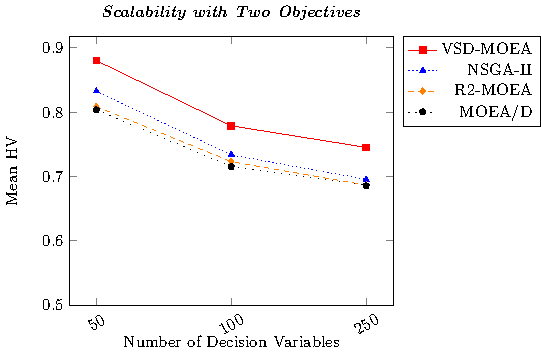
\includegraphics[]{Images/Graphic-Scalability-2obj_tikz-figure0.pdf}
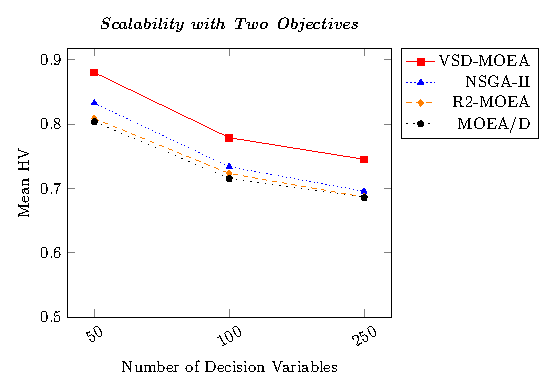
\includegraphics[]{Images/Graphic-Scalability-2obj_tikz-figure0.eps}
%\begin{tikzpicture}[scale=0.8]
\begin{axis}[
ymin=0.5,
%ymax=1.1,
%x label style={at={(current axis.left of origin)},anchor=north, below=10mm},
title={\textit{\textbf{Scalability with Two Objectives}}},
    xlabel=Number of Decision Variables,
  ylabel=Mean HV,
%  xlabel style={yshift=-0.2cm},
  xticklabel style = {rotate=30},
  legend style=
    {cells={anchor=east},legend pos=outer north east,},
  % enlargelimits = false,
  xticklabels from table={\ScalabilityTwoObj}{mean},xtick=data]
  
\addplot[red,solid,mark=square*] 
table [y=VSD_MOEA,x=X]{\ScalabilityTwoObj};
\addlegendentry{VSD-MOEA}
\addplot[blue,dotted,mark=triangle*] table[y= CPDEA,x=X]{\ScalabilityTwoObj};
\addlegendentry{CPDEA}]
		
\addplot[orange,dashed,mark=diamond*] table [y= R2_MOEA,x=X]{\ScalabilityTwoObj};
\addlegendentry{R2-EMOA}]
    
\addplot[black,loosely dotted,mark=pentagon*] table [y= MOEA_D,x=X]{\ScalabilityTwoObj};
\addlegendentry{MOEA/D}]
\end{axis}
\end{tikzpicture}
%\begin{tikzpicture}[scale=0.8]
%\begin{axis}[
%%ymin=0.5    ,
%%ymax=1.1,
%%x label style={at={(current axis.left of origin)},anchor=north, below=10mm},
%title={\textit{\textbf{Scalability UF5}}},
%    xlabel=Number of Decision Variables,
%  ylabel=Mean HV,
%  xticklabel style = {rotate=30},
%  legend style=
%    {cells={anchor=east},legend pos=outer north east,},
%  % enlargelimits = false,
%  xticklabels from table={\ScalabilityUFFiveTwoObj}{mean},xtick=data]
%  
%\addplot[red,solid,mark=square*] 
%table [y=VSD_MOEA,x=X]{\ScalabilityUFFiveTwoObj};
%\addlegendentry{VSD-MOEA}
%\addplot[blue,dotted,mark=triangle*] table [y= NSGA_II,x=X]{\ScalabilityUFFiveTwoObj};
%\addlegendentry{NSGA-II}]
%		
%\addplot[orange,dashed,mark=diamond*] table [y= R2_MOEA,x=X]{\ScalabilityUFFiveTwoObj};
%\addlegendentry{R2-MOEA}]
%    
%\addplot[black,loosely dotted,mark=pentagon*] table [y= MOEA_D,x=X]{\ScalabilityUFFiveTwoObj};
%\addlegendentry{MOEA/D}]
%\end{axis}
%\end{tikzpicture}
%\caption{Mean of the \HV{} (35 runs) considering two objectives.}

\caption{Mean of the ratio \HV{} of 35 runs and considering two objectives.}\label{fig:variable-decision-scalability-2obj}
\end{figure}

\begin{figure}[t]
\centering
%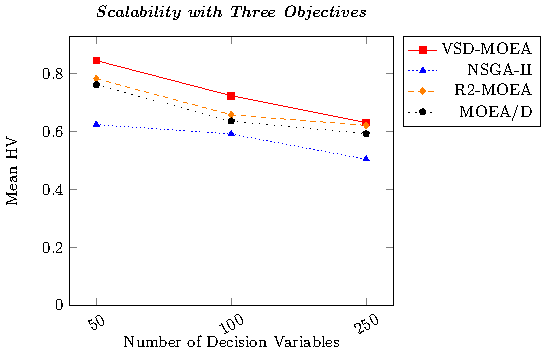
\includegraphics[]{Images/Graphic-Scalability-3obj_tikz-figure0.pdf}
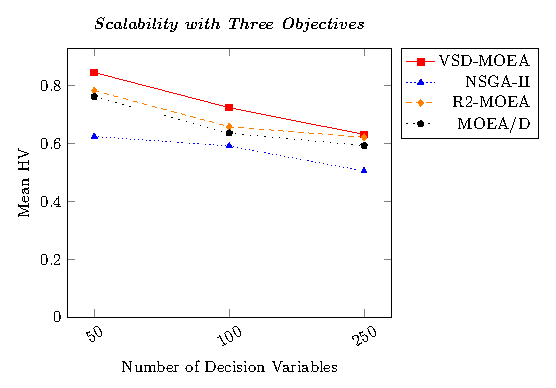
\includegraphics[]{Images/Graphic-Scalability-3obj_tikz-figure0.eps}
%\begin{tikzpicture}[scale=0.8]
\begin{axis}[
ymin=0.0,
title={\textit{\textbf{Scalability with Three Objectives}}},
    xlabel=Number of Decision Variables,
  ylabel=Mean HV,
%  xlabel style={yshift=-0.2cm},
  xticklabel style = {rotate=30},
  legend style=
    {cells={anchor=east},legend pos=outer north east,},
  xticklabels from table={\ScalabilityThreeObj}{mean},xtick=data]
  
\addplot[red,solid,mark=square*] 
table [y=VSD_MOEA,x=X]{\ScalabilityThreeObj};
\addlegendentry{VSD-MOEA}
\addplot[blue,dotted,mark=triangle*] table [y= NSGA_II,x=X]{\ScalabilityThreeObj};
\addlegendentry{NSGA-II}]
		
\addplot[orange,dashed,mark=diamond*] table [y= R2_MOEA,x=X]{\ScalabilityThreeObj};
\addlegendentry{R2-EMOA}]
    
\addplot[black,loosely dotted,mark=pentagon*] table [y= MOEA_D,x=X]{\ScalabilityThreeObj};
\addlegendentry{MOEA/D}]
\end{axis}
\end{tikzpicture}
%\begin{tikzpicture}[scale=0.8]
%\begin{axis}[
%ymin=0.0,
%title={\textit{\textbf{Scalability UF10}}},
%    xlabel=Number of Decision Variables,
%  ylabel=Mean HV,
%  xticklabel style = {rotate=30},
%  legend style=
%    {cells={anchor=east},legend pos=outer north east,},
%  xticklabels from table={\ScalabilityUFTenThreeObj}{mean},xtick=data]
%  
%\addplot[red,solid,mark=square*] 
%table [y=VSD_MOEA,x=X]{\ScalabilityUFTenThreeObj};
%\addlegendentry{VSD-MOEA}
%\addplot[blue,dotted,mark=triangle*] table [y= NSGA_II,x=X]{\ScalabilityUFTenThreeObj};
%\addlegendentry{NSGA-II}]
%		
%\addplot[orange,dashed,mark=diamond*] table [y= R2_MOEA,x=X]{\ScalabilityUFTenThreeObj};
%\addlegendentry{R2-MOEA}]
%    
%\addplot[black,loosely dotted,mark=pentagon*] table [y= MOEA_D,x=X]{\ScalabilityUFTenThreeObj};
%\addlegendentry{MOEA/D}]
%\end{axis}
%\end{tikzpicture}
%\caption{Mean of the \HV{} (35 runs) considering three objectives.}

\caption{Mean of the ratio \HV{} of 35 runs and considering three objectives.} \label{fig:variable-decision-scalability-3obj}
\end{figure}

In order to better understand this behaviour, we selected the WFG1 to WFG7 problems.
%
WFG problems divide the decision variables in two kinds of parameters: the distance parameters and the position parameters.
%
Note that, a parameter $i$ is a distance parameter when for all $\vec{\mathbf{x}}$, modifying $x_i$ results in a new solution 
that dominates $\vec{\mathbf{x}}$, is equivalent to $\vec{\mathbf{x}}$, or is dominated by $\vec{\mathbf{x}}$.
%
However, if $i$ is a position parameter, modifying $x_i$ in $\vec{\mathbf{x}}$ always results in a vector that is incomparable or 
equivalent to $\vec{\mathbf{x}}$~\cite{huband2005scalable}.
%
Additionally, note that we selected the WFG1-WFG7 problems because their distance parameters values associated to all Pareto optimal solutions 
have exactly the same values.
%
This values is shown as follows:
\begin{equation}
   x_{i=k+1:n} = 2i \times 0.35
\end{equation}
%
This is really important because it has been shown that for some cases, state-of-the-art
\MOEAS{} provoke a quick convergence in \textit{distance parameters}, resulting in an effect that is similar to premature convergence
in the single-objective case.

For each algorithms, we calculated the avarege Euclidean distance among individuals (ADI) in the population by considering only 
the distance parameters.
%
Figures \ref{fig:Diversity_2obj} and \ref{fig:Diversity_3obj} shows the ADI evolution for the two-objective and three-objective problems.
%
In order to not sature this Figures, only the information of \VSDMOEA{} and \RMOEA{} with 50, 100 and 250 decision variables is shown.

%
The first evident issue is that \VSDMOEA{} converges much slower than \RMOEA{}.
%
In this way, the difference between the diversity maintained in the first generation and the one maintained after 10\% of the execution,
is much larger in \RMOEA{} than in \VSDMOEA{}.
%
In the case of \VSDMOEA{}, the decrease in ADI is quite linear until the 50\% of the execution.
%
This is due to the way in which the threshold distance value ($D_t$) is calculated.
%
Additionally, when inspecting more closely the data, some other important aspects must be discussed. 
%
In the two-objective case, increasing the number of variables provokes a slight increase on the diversity in \RMOEA{}.
%
However, the amount of diversity is low even when using 250 distance variables, meaning that incorporating mechanisms to increase diversity --- as it is done in \VSDMOEA{} ---
is really helpful.
%
Differently, in the three-objective case, the amount of diversity in \RMOEA{} is not so low.
%
Moreover, increasing the number of decision variables, provokes an important increase in the attained ADI, meaning that in this case,
fast convergence is not an issue.
%
These results show that, as the number of objectives and variables increases, \MOEAS{} tend to maintain a higher variable space diversity
in an implicity way, meaning that explicitly controlling the variable space diversity is probably not so important.
%
Note that the behaviour of \NSGAII{} and \MOEAD{} in terms of the ADI evolution is similar to the one analyzed for \RMOEA{}.

Finally, we would like to note that we selected some specific problems to perform long-term executions with 250 distance variables.
%
\VSDMOEA{} could improve further the results when using long-term executions, while the other state-of-the-art algorithms dit not attain
important improvements.
%
This probably means that as the technology evolves and longer executions (more generations) can be performed in admisible times,
the incorporation of explicit control of diversity will be even more important.
%
Note that this also happens in the single-objective case, where benefits of explicit control of diversity appears only when using executions of
several weeks when dealing with large instances of the Traveling Salesman Problem~\cite{segura2015novel}.
%



\begin{figure}[t]
\centering
%\begin{tikzpicture}[scale=0.8]
\begin{axis}[
title={\textit{\textbf{Diversity of the Position Variables with Two Objectives}}},
  xlabel=Generation,
  ylabel=ADI,
  xticklabel style = {rotate=30},
%  xlabel style={yshift=-0.2cm},
  legend style=
    {cells={anchor=east},legend pos=outer north east,}, nodes={scale=0.8, transform shape}    ,
  xticklabels from table={\DiversityTwoWFG}{mean},xtick=data]
 

\addplot[red,dotted,mark=square*] table [y=VSD_MOEA_Position_50,x=X]{\DiversityTwoWFG};
	\addlegendentry{VSD-MOEA (50)}

\addplot[blue,dotted,mark=triangle*] table[y= NSGA_II_Position_50,x=X]{\DiversityTwoWFG};
	\addlegendentry{NSGA-II (50)}
		
\addplot[orange,dotted,mark=diamond*] table [y= R2_MOEA_Position_50,x=X]{\DiversityTwoWFG};
	\addlegendentry{R2-EMOA (50)}
    
\addplot[black,dotted,mark=pentagon*] table [y= MOEA_D_Position_50,x=X]{\DiversityTwoWFG};
	\addlegendentry{MOEA/D (50)}


\addplot[red,solid,mark=square*] table [y=VSD_MOEA_Position_100,x=X]{\DiversityTwoWFG};
	\addlegendentry{VSD-MOEA (100)}

\addplot[blue,solid,mark=triangle*] table[y= NSGA_II_Position_100,x=X]{\DiversityTwoWFG};
	\addlegendentry{NSGA-II (100)}
		
\addplot[orange,solid,mark=diamond*] table [y= R2_MOEA_Position_100,x=X]{\DiversityTwoWFG};
	\addlegendentry{R2-EMOA (100)}
    
\addplot[black,solid,mark=pentagon*] table [y= MOEA_D_Position_100,x=X]{\DiversityTwoWFG};
	\addlegendentry{MOEA/D (100)}


\addplot[red,loosely dashdotted,mark=square*] table [y=VSD_MOEA_Position_250,x=X]{\DiversityTwoWFG};
	\addlegendentry{VSD-MOEA (250)}

\addplot[blue,loosely dashdotted,mark=triangle*] table[y= NSGA_II_Position_250,x=X]{\DiversityTwoWFG};
	\addlegendentry{NSGA-II (250)}
		
\addplot[orange,loosely dashdotted,mark=diamond*] table [y= R2_MOEA_Position_250,x=X]{\DiversityTwoWFG};
	\addlegendentry{R2-EMOA (250)}
    
\addplot[black,loosely dashdotted,mark=pentagon*] table [y= MOEA_D_Position_250,x=X]{\DiversityTwoWFG};
	\addlegendentry{MOEA/D (250)}



\end{axis}
\end{tikzpicture}


\begin{tikzpicture}[scale=0.8]
\begin{axis}[
title={\textit{\textbf{Diversity of the Distance Variables with Two Objectives}}},
  xlabel=Generation,
  ylabel=ADI,
%  xlabel style={yshift=-0.2cm},
  xticklabel style = {rotate=30},
  legend style=
    {cells={anchor=east},legend pos=outer north east,}, nodes={scale=0.8, transform shape}    ,
  xticklabels from table={\DiversityTwoWFG}{mean},xtick=data]

\addplot[red,dotted,mark=square*] table [y=VSD_MOEA_Distance_50,x=X]{\DiversityTwoWFG};
	\addlegendentry{VSD-MOEA (50)}

%\addplot[blue,dotted,mark=triangle*] table[y= NSGA_II_Distance_50,x=X]{\DiversityTwoWFG};
%	\addlegendentry{NSGA-II (50)}
		
\addplot[orange,dotted,mark=diamond*] table [y= R2_MOEA_Distance_50,x=X]{\DiversityTwoWFG};
	\addlegendentry{R2-EMOA (50)}
    
%\addplot[black,dotted,mark=pentagon*] table [y= MOEA_D_Distance_50,x=X]{\DiversityTwoWFG};
%	\addlegendentry{MOEA/D (50)}


\addplot[red,solid,mark=square*] table [y=VSD_MOEA_Distance_100,x=X]{\DiversityTwoWFG};
	\addlegendentry{VSD-MOEA (100)}

%\addplot[blue,solid,mark=triangle*] table[y= NSGA_II_Distance_100,x=X]{\DiversityTwoWFG};
%	\addlegendentry{NSGA-II (100)}
		
\addplot[orange,solid,mark=diamond*] table [y= R2_MOEA_Distance_100,x=X]{\DiversityTwoWFG};
	\addlegendentry{R2-EMOA (100)}
    
%\addplot[black,solid,mark=pentagon*] table [y= MOEA_D_Distance_100,x=X]{\DiversityTwoWFG};
%	\addlegendentry{MOEA/D (100)}


\addplot[red,loosely dashdotted,mark=square*] table [y=VSD_MOEA_Distance_250,x=X]{\DiversityTwoWFG};
	\addlegendentry{VSD-MOEA (250)}

%\addplot[blue,loosely dashdotted,mark=triangle*] table[y= NSGA_II_Distance_250,x=X]{\DiversityTwoWFG};
%	\addlegendentry{NSGA-II (250)}
		
\addplot[orange,loosely dashdotted,mark=diamond*] table [y= R2_MOEA_Distance_250,x=X]{\DiversityTwoWFG};
	\addlegendentry{R2-EMOA (250)}
    
%\addplot[black,loosely dashdotted,mark=pentagon*] table [y= MOEA_D_Distance_250,x=X]{\DiversityTwoWFG};
%	\addlegendentry{MOEA/D (250)}





\end{axis}
\end{tikzpicture}

%%\begin{tikzpicture}[scale=0.8]
%%\begin{axis}[
%%title={\textit{\textbf{Diversity of the Variables}}},
%%  xlabel=Generation,
%%  ylabel=ADI,
%%  xticklabel style = {rotate=30},
%%  legend style=
%%    {cells={anchor=east},legend pos=outer north east,},
%%  xticklabels from table={\DiversityTwoWFGOne}{mean},xtick=data]
%%
%%\addplot[red,dotted,mark=square*] table [y=VSD_MOEA,x=X]{\DiversityTwoWFGOne};
%%\addlegendentry{VSD-MOEA}
%%
%%\addplot[blue,dotted,mark=triangle*] table[y= NSGA_II,x=X]{\DiversityTwoWFGOne};
%%\addlegendentry{NSGA-II}
%%		
%%\addplot[orange,dotted,mark=diamond*] table [y= R2_MOEA,x=X]{\DiversityTwoWFGOne};
%%\addlegendentry{R2-MOEA}
%%    
%%\addplot[black,dotted,mark=pentagon*] table [y= MOEA_D,x=X]{\DiversityTwoWFGOne};
%%\addlegendentry{MOEA/D}
%%
%%
%%\addplot[red,solid,mark=square*] table [y=VSD_MOEA,x=X]{\DiversityThreeWFGOne};
%%\addlegendentry{VSD-MOEA}
%%
%%\addplot[blue,solid,mark=triangle*] table[y= NSGA_II,x=X]{\DiversityThreeWFGOne};
%%\addlegendentry{NSGA-II}
%%		
%%\addplot[orange,solid,mark=diamond*] table [y= R2_MOEA,x=X]{\DiversityThreeWFGOne};
%%\addlegendentry{R2-MOEA}
%%    
%%\addplot[black,solid,mark=pentagon*] table [y= MOEA_D,x=X]{\DiversityThreeWFGOne};
%%\addlegendentry{MOEA/D}
%%
%%	
%%\end{axis}
%%\end{tikzpicture}
%\caption{Evolution of Average Distance Individuals of the Problems WFG1-WFG7.}


%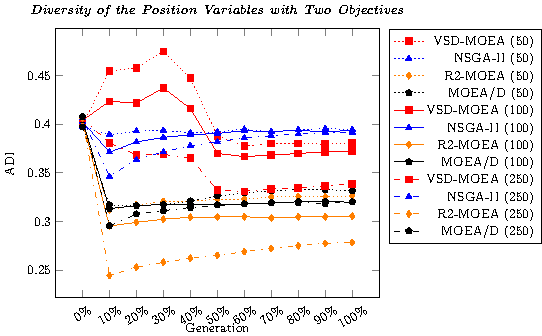
\includegraphics[]{Images/Graphic-Diversity_2obj_tikz-figure0.pdf} \\
%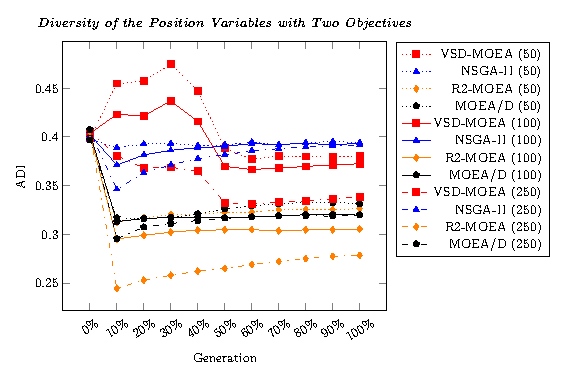
\includegraphics[]{Images/Graphic-Diversity_2obj_tikz-figure0.eps} \\[0.2cm]
%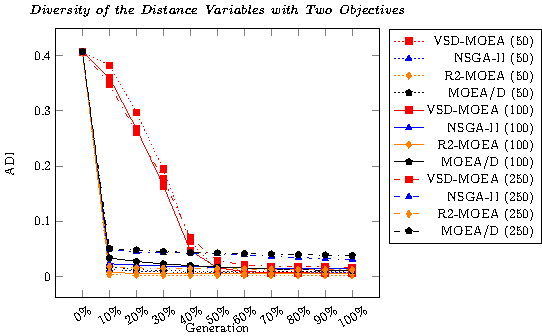
\includegraphics[]{Images/Graphic-Diversity_2obj_tikz-figure1.pdf}
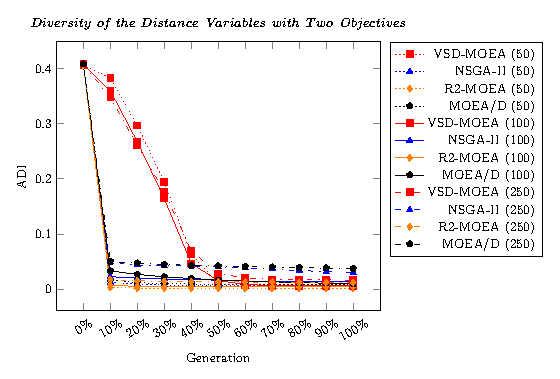
\includegraphics[]{Images/Graphic-Diversity_2obj_tikz-figure1.eps}
\caption{Evolution of ADI for the problems WFG1-WFG7 with two objectives.}\label{fig:Diversity_2obj}
\end{figure}



%
%

\begin{figure}[t]
\centering
%\begin{tikzpicture}[scale=0.8]
\begin{axis}[
title={\textit{\textbf{Diversity of the Position Variables with Three Objectives}}},
  xlabel=Function Evaluations,
  ylabel=ADI,
%  xlabel style={yshift=-0.2cm},
 xticklabel style = {rotate=30},
  legend style=
   {cells={anchor=east},legend pos=outer north east,}, nodes={scale=0.8, transform shape}    ,
    %{cells={anchor=east},legend pos=outer north east,},
  xticklabels from table={\DiversityThreeWFG}{mean},xtick=data]
 

\addplot[red,dotted,mark=square*] table [y=VSD_MOEA_Position_50,x=X]{\DiversityThreeWFG};
	\addlegendentry{VSD-MOEA (50)}

\addplot[blue,dotted,mark=triangle*] table[y= CPDEA_Position_50,x=X]{\DiversityThreeWFG};
	\addlegendentry{CPDEA (50)}
		
\addplot[orange,dotted,mark=diamond*] table [y= R2_MOEA_Position_50,x=X]{\DiversityThreeWFG};
	\addlegendentry{R2-EMOA (50)}
    
\addplot[black,dotted,mark=pentagon*] table [y= MOEA_D_Position_50,x=X]{\DiversityThreeWFG};
	\addlegendentry{MOEA/D (50)}


\addplot[red,solid,mark=square*] table [y=VSD_MOEA_Position_100,x=X]{\DiversityThreeWFG};
	\addlegendentry{VSD-MOEA (100)}

\addplot[blue,solid,mark=triangle*] table[y= CPDEA_Position_100,x=X]{\DiversityThreeWFG};
	\addlegendentry{CPDEA (100)}
		
\addplot[orange,solid,mark=diamond*] table [y= R2_MOEA_Position_100,x=X]{\DiversityThreeWFG};
	\addlegendentry{R2-EMOA (100)}
    
\addplot[black,solid,mark=pentagon*] table [y= MOEA_D_Position_100,x=X]{\DiversityThreeWFG};
	\addlegendentry{MOEA/D (100)}


\addplot[red,loosely dashdotted,mark=square*] table [y=VSD_MOEA_Position_250,x=X]{\DiversityThreeWFG};
	\addlegendentry{VSD-MOEA (250)}

\addplot[blue,loosely dashdotted,mark=triangle*] table[y= CPDEA_Position_250,x=X]{\DiversityThreeWFG};
	\addlegendentry{CPDEA (250)}
		
\addplot[orange,loosely dashdotted,mark=diamond*] table [y= R2_MOEA_Position_250,x=X]{\DiversityThreeWFG};
	\addlegendentry{R2-EMOA (250)}
    
\addplot[black,loosely dashdotted,mark=pentagon*] table [y= MOEA_D_Position_250,x=X]{\DiversityThreeWFG};
	\addlegendentry{MOEA/D (250)}



\end{axis}
\end{tikzpicture}


\begin{tikzpicture}[scale=0.8]
\begin{axis}[
title={\textit{\textbf{Diversity of the Distance Variables with Three Objectives}}},
  xlabel=Function Evaluations,
  ylabel=ADI,
	ymax=0.6,
  xticklabel style = {rotate=30},
   ytick={ 0, 0.1, 0.2, 0.3, 0.4, 0.5, 0.6},
%  xlabel style={yshift=-0.2cm},
  legend style=
   {cells={anchor=east},legend pos=outer north east,}, nodes={scale=0.8, transform shape}    ,
    %{cells={anchor=east},legend pos=outer north east,},
  xticklabels from table={\DiversityThreeWFG}{mean},xtick=data]

\addplot[red,dotted,mark=square*] table [y=VSD_MOEA_Distance_50,x=X]{\DiversityThreeWFG};
	\addlegendentry{VSD-MOEA (50)}

\addplot[blue,dotted,mark=triangle*] table[y= CPDEA_Distance_50,x=X]{\DiversityThreeWFG};
	\addlegendentry{CPDEA (50)}
		
\addplot[orange,dotted,mark=diamond*] table [y= R2_MOEA_Distance_50,x=X]{\DiversityThreeWFG};
	\addlegendentry{R2-EMOA (50)}
    
%\addplot[black,dotted,mark=pentagon*] table [y= MOEA_D_Distance_50,x=X]{\DiversityThreeWFG};
%	\addlegendentry{MOEA/D (50)}


%\addplot[red,solid,mark=square*] table [y=VSD_MOEA_Distance_100,x=X]{\DiversityThreeWFG};
%	\addlegendentry{VSD-MOEA (100)}

%\addplot[blue,solid,mark=triangle*] table[y= CPDEA_Distance_100,x=X]{\DiversityThreeWFG};
%	\addlegendentry{CPDEA (100)}
		
%\addplot[orange,solid,mark=diamond*] table [y= R2_MOEA_Distance_100,x=X]{\DiversityThreeWFG};
%	\addlegendentry{R2-EMOA (100)}
    
%\addplot[black,solid,mark=pentagon*] table [y= MOEA_D_Distance_100,x=X]{\DiversityThreeWFG};
%	\addlegendentry{MOEA/D (100)}


\addplot[red,loosely dashdotted,mark=square*] table [y=VSD_MOEA_Distance_250,x=X]{\DiversityThreeWFG};
	\addlegendentry{VSD-MOEA (250)}

\addplot[blue,loosely dashdotted,mark=triangle*] table[y= CPDEA_Distance_250,x=X]{\DiversityThreeWFG};
	\addlegendentry{CPDEA (250)}
		
\addplot[orange,loosely dashdotted,mark=diamond*] table [y= R2_MOEA_Distance_250,x=X]{\DiversityThreeWFG};
	\addlegendentry{R2-EMOA (250)}
    
%\addplot[black,loosely dashdotted,mark=pentagon*] table [y= MOEA_D_Distance_250,x=X]{\DiversityThreeWFG};
%	\addlegendentry{MOEA/D (250)}





\end{axis}
\end{tikzpicture}

%%\begin{tikzpicture}[scale=0.8]
%%\begin{axis}[
%%title={\textit{\textbf{Diversity of the Variables}}},
%%  xlabel=Generation,
%%  ylabel=ADI,
%%  xticklabel style = {rotate=30},
%%  legend style=
%%    {cells={anchor=east},legend pos=outer north east,},
%%  xticklabels from table={\DiversityThreeWFGOne}{mean},xtick=data]
%%
%%\addplot[red,dotted,mark=square*] table [y=VSD_MOEA,x=X]{\DiversityThreeWFGOne};
%%\addlegendentry{VSD-MOEA}
%%
%%\addplot[blue,dotted,mark=triangle*] table[y= CPDEA,x=X]{\DiversityThreeWFGOne};
%%\addlegendentry{CPDEA}
%%		
%%\addplot[orange,dotted,mark=diamond*] table [y= R2_MOEA,x=X]{\DiversityThreeWFGOne};
%%\addlegendentry{R2-MOEA}
%%    
%%\addplot[black,dotted,mark=pentagon*] table [y= MOEA_D,x=X]{\DiversityThreeWFGOne};
%%\addlegendentry{MOEA/D}
%%
%%
%%\addplot[red,solid,mark=square*] table [y=VSD_MOEA,x=X]{\DiversityThreeWFGOne};
%%\addlegendentry{VSD-MOEA}
%%
%%\addplot[blue,solid,mark=triangle*] table[y= CPDEA,x=X]{\DiversityThreeWFGOne};
%%\addlegendentry{CPDEA}
%%		
%%\addplot[orange,solid,mark=diamond*] table [y= R2_MOEA,x=X]{\DiversityThreeWFGOne};
%%\addlegendentry{R2-MOEA}
%%    
%%\addplot[black,solid,mark=pentagon*] table [y= MOEA_D,x=X]{\DiversityThreeWFGOne};
%%\addlegendentry{MOEA/D}
%%
%%	
%%\end{axis}
%%\end{tikzpicture}
%\caption{Evolution of Average Distance Individuals of the Problems WFG1-WFG7.}

%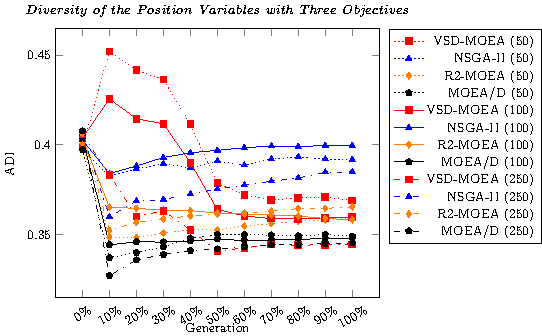
\includegraphics[]{Images/Graphic-Diversity_3obj_tikz-figure0.pdf} \\
%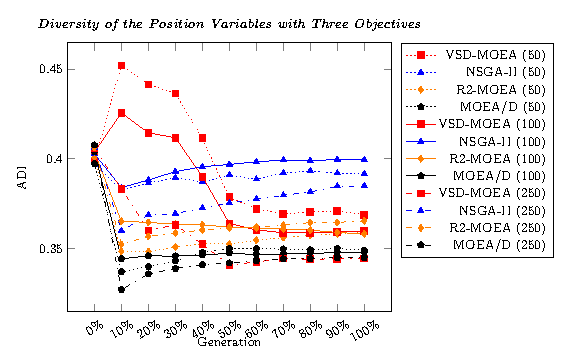
\includegraphics[]{Images/Graphic-Diversity_3obj_tikz-figure0.eps} \\[0.2cm]
%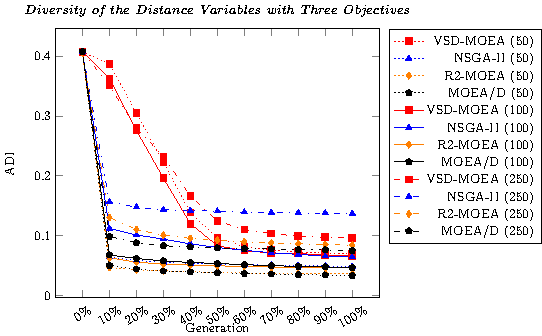
\includegraphics[]{Images/Graphic-Diversity_3obj_tikz-figure1.pdf}
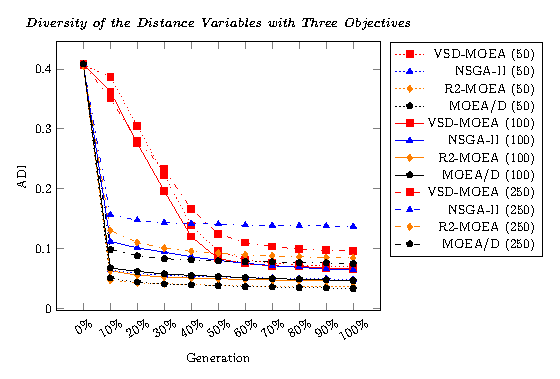
\includegraphics[]{Images/Graphic-Diversity_3obj_tikz-figure1.eps}
\caption{Evolution of ADI for the problems WFG1-WFG7 with three objectives.}\label{fig:Diversity_3obj}
\end{figure}
%\begin{figure}[t]
%\centering
%\begin{tikzpicture}[scale=0.8]
\begin{axis}[
title={\textit{\textbf{Diversity of the Position Variables}}},
  xlabel=Generation,
  ylabel=ADI,
  xticklabel style = {rotate=30},
  legend style=
    {cells={anchor=east},legend pos=outer north east,},
  xticklabels from table={\DiversityTwoWFGSix}{mean},xtick=data]
 

\addplot[red,dotted,mark=square*] table [y=VSD_MOEA_Position,x=X]{\DiversityTwoWFGSix};
\addlegendentry{VSD-MOEA}

\addplot[blue,dotted,mark=triangle*] table[y= NSGA_II_Position,x=X]{\DiversityTwoWFGSix};
\addlegendentry{NSGA-II}
		
\addplot[orange,dotted,mark=diamond*] table [y= R2_MOEA_Position,x=X]{\DiversityTwoWFGSix};
\addlegendentry{R2-MOEA}
    
\addplot[black,dotted,mark=pentagon*] table [y= MOEA_D_Position,x=X]{\DiversityTwoWFGSix};
\addlegendentry{MOEA/D}


\addplot[red,solid,mark=square*] table [y=VSD_MOEA_Position,x=X]{\DiversityThreeWFGSix};
\addlegendentry{VSD-MOEA}

\addplot[blue,solid,mark=triangle*] table[y= NSGA_II_Position,x=X]{\DiversityThreeWFGSix};
\addlegendentry{NSGA-II}
		
\addplot[orange,solid,mark=diamond*] table [y= R2_MOEA_Position,x=X]{\DiversityThreeWFGSix};
\addlegendentry{R2-MOEA}
    
\addplot[black,solid,mark=pentagon*] table [y= MOEA_D_Position,x=X]{\DiversityThreeWFGSix};
\addlegendentry{MOEA/D}


\end{axis}
\end{tikzpicture}


\begin{tikzpicture}[scale=0.8]
\begin{axis}[
title={\textit{\textbf{Diversity of the Distance Variables}}},
  xlabel=Generation,
  ylabel=ADI,
  xticklabel style = {rotate=30},
  legend style=
    {cells={anchor=east},legend pos=outer north east,},
  xticklabels from table={\DiversityTwoWFGSix}{mean},xtick=data]

\addplot[red,dotted,mark=square*] table [y=VSD_MOEA_Distance,x=X]{\DiversityTwoWFGSix};
\addlegendentry{VSD-MOEA}

\addplot[blue,dotted,mark=triangle*] table[y= NSGA_II_Distance,x=X]{\DiversityTwoWFGSix};
\addlegendentry{NSGA-II}
		
\addplot[orange,dotted,mark=diamond*] table [y= R2_MOEA_Distance,x=X]{\DiversityTwoWFGSix};
\addlegendentry{R2-MOEA}
    
\addplot[black,dotted,mark=pentagon*] table [y= MOEA_D_Distance,x=X]{\DiversityTwoWFGSix};
\addlegendentry{MOEA/D}


\addplot[red,solid,mark=square*] table [y=VSD_MOEA_Distance,x=X]{\DiversityThreeWFGSix};
\addlegendentry{VSD-MOEA}

\addplot[blue,solid,mark=triangle*] table[y= NSGA_II_Distance,x=X]{\DiversityThreeWFGSix};
\addlegendentry{NSGA-II}
		
\addplot[orange,solid,mark=diamond*] table [y= R2_MOEA_Distance,x=X]{\DiversityThreeWFGSix};
\addlegendentry{R2-MOEA}
    
\addplot[black,solid,mark=pentagon*] table [y= MOEA_D_Distance,x=X]{\DiversityThreeWFGSix};
\addlegendentry{MOEA/D}

	
\end{axis}
\end{tikzpicture}

\begin{tikzpicture}[scale=0.8]
\begin{axis}[
title={\textit{\textbf{Diversity of the Variables}}},
  xlabel=Generation,
  ylabel=ADI,
  xticklabel style = {rotate=30},
  legend style=
    {cells={anchor=east},legend pos=outer north east,},
  xticklabels from table={\DiversityTwoWFGSix}{mean},xtick=data]

\addplot[red,dotted,mark=square*] table [y=VSD_MOEA,x=X]{\DiversityTwoWFGSix};
\addlegendentry{VSD-MOEA}

\addplot[blue,dotted,mark=triangle*] table[y= NSGA_II,x=X]{\DiversityTwoWFGSix};
\addlegendentry{NSGA-II}
		
\addplot[orange,dotted,mark=diamond*] table [y= R2_MOEA,x=X]{\DiversityTwoWFGSix};
\addlegendentry{R2-MOEA}
    
\addplot[black,dotted,mark=pentagon*] table [y= MOEA_D,x=X]{\DiversityTwoWFGSix};
\addlegendentry{MOEA/D}


\addplot[red,solid,mark=square*] table [y=VSD_MOEA,x=X]{\DiversityThreeWFGSix};
\addlegendentry{VSD-MOEA}

\addplot[blue,solid,mark=triangle*] table[y= NSGA_II,x=X]{\DiversityThreeWFGSix};
\addlegendentry{NSGA-II}
		
\addplot[orange,solid,mark=diamond*] table [y= R2_MOEA,x=X]{\DiversityThreeWFGSix};
\addlegendentry{R2-MOEA}
    
\addplot[black,solid,mark=pentagon*] table [y= MOEA_D,x=X]{\DiversityThreeWFGSix};
\addlegendentry{MOEA/D}

	
\end{axis}
\end{tikzpicture}

\caption{Evolution of the diversity for the problem WFG6}


%\label{fig:Diversity_WFG6}
%\end{figure}

\subsection{Stopping criteria and Diversity}

As previously discussed, \EAS{} with explicit control of diversity are usually more useful in long-term executions.
%
Since in our first experiment we selected a quite large stopping criterion, reader might consider that \VSDMOEA{} is only
useful in really long-term executions.
%
However, this is not the case.
%
This section is devoted to analyze the performance of \VSDMOEA{} and state-of-the-art algorithms with several stopping criteria, 
i.e. maximum number of generations.
%
Three different ranges of stopping criterion were explored.
%
Each range was split in ten intervals equally distributed and experiments with each differnet number of generations were run.
%
Note that state-of-the-art algorithms can be executed just one time (with $250,000$ generations) by saving the intermediate results.
%
However, \VSDMOEA{} takes decisions that depend on the stopping criteria, so independent executions were required for each stopping criterion.
%
The ranges considered were $[250, 2500]$, $[2500, 25000]$ and $[25000, 250000]$.
%
These ranges are referred to as short-term, middle-term and long-term executions, respectively.

Figures \ref{fig:Performance_time_2obj} and \ref{fig:Performance_time_3obj} show the mean \HV{} ratio attained with each \MOEA{} with two and three objectives respectively.
%
To calculate this mean ratio, all the problems are considered simultaneously configured as in the first described experiment.
%
Each figure is divided in three graphics corresponding to short-term, middle-term and long-term.
%
In the two-objective case, for the shortest executions \VSDMOEA{} is not very competitive.
%
In the range $[250, 750]$ presents the last performance, meaning that for really short-term executions,
explicitly promoting additional diversity is not helpful.
%
In the case of using $1,000$ generations, the attained \HV{} ratio is similar than the one attained by other methods.
%
Finally, when using more than $925$ generations, the \HV{} ratio attained by \VSDMOEA{} is much larger than the one
attained by other methods.
%
It is noticeable that \VSDMOEA{} is the only method that really takes advantages of using long-term executions,
with the remaining methods just showing a slight improvement.
%
In the three-objective case, \VSDMOEA{} attains a lower \HV{} ratio than \RMOEA{} and \MOEAD{} in short-term executions,
but as more generations are granted, the differences decrease.
%
In this case, when $5,000$ generations are evolved, the performance of \VSDMOEA{} is similar to the one of \RMOEA{}.
%
Finally, as in the two-objective case, with more generations the differences between \VSDMOEA{} and the remaining
algorithms increase in favor of \VSDMOEA{}.
%
Thus, while the most important benefits arise in long-term executions, practitioners can benefit from the use
of \VSDMOEA{} even in shorter executions.


\begin{figure}[t]
\centering
%\begin{tikzpicture}[scale=0.8]
\begin{axis}[
title={\textit{\textbf{Performance of \MOEAS{} with Two Objectives}}},
  xlabel= Maximum Number of Generations,
  ylabel=Mean HV,
%  ymin=0.3,
  ymax=1.0,
  xticklabel style = {rotate=90, anchor=east, font=\footnotesize,},
%  label style = {font=\small, },
%xlabel style={yshift=-1cm},
%  xmode=log,
%  log basis x={2},
  legend style=
    {cells={anchor=east},legend pos=outer north east,},
  xticklabels from table={\Performancetimetwo}{mean},xtick=data]
 

\addplot[red,dotted,mark=square*] table [y=VSD_MOEA,x=X]{\Performancetimetwo};
\addlegendentry{VSD-MOEA}

\addplot[blue,dotted,mark=triangle*] table[y= NSGA_II,x=X]{\Performancetimetwo};
\addlegendentry{NSGA-II}
		
\addplot[orange,dotted,mark=diamond*] table [y= R2_MOEA,x=X]{\Performancetimetwo};
\addlegendentry{R2-MOEA}
    
\addplot[black,dotted,mark=pentagon*] table [y= MOEA_D,x=X]{\Performancetimetwo};
\addlegendentry{MOEA/D}
\draw [red, dashed] (axis cs:10, 0) -- (axis cs:10, 1);
\draw [red, dashed] (axis cs:19, 0) -- (axis cs:19, 1);
\end{axis}
\end{tikzpicture}


\begin{tikzpicture}[scale=0.8]
\begin{axis}[
title={\textit{\textbf{Performance of \MOEAS{} with Three Objectives}}},
  xlabel= Maximum Number of Generations,
  ylabel=Mean HV,
%  ymin=0.5,
 % ymax=1.0,
  xticklabel style = {rotate=90, anchor=east, font=\footnotesize,},
  legend style=
    {cells={anchor=east},legend pos=outer north east,},
  xticklabels from table={\Performancetimethree}{mean},xtick=data]

\addplot[red,dashed,mark=square*] table [y=VSD_MOEA,x=X]{\Performancetimethree};
\addlegendentry{VSD-MOEA}

\addplot[blue,dashed,mark=triangle*] table[y= NSGA_II,x=X]{\Performancetimethree};
\addlegendentry{NSGA-II}
		
\addplot[orange,dashed,mark=diamond*] table [y= R2_MOEA,x=X]{\Performancetimethree};
\addlegendentry{R2-MOEA}
    
\addplot[black,dashed,mark=pentagon*] table [y= MOEA_D,x=X]{\Performancetimethree};
\addlegendentry{MOEA/D};
\draw [red, dashed] (axis cs:10, 0) -- (axis cs:10, 1);
\draw [red, dashed] (axis cs:19, 0) -- (axis cs:19, 1);
\end{axis}
\end{tikzpicture}



\caption{Performance of the \MOEAS{} considerin several maximum number of generations.}

%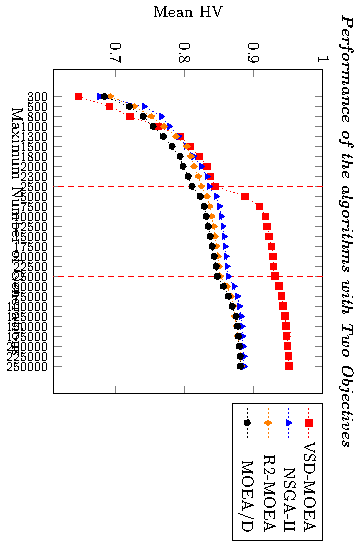
\includegraphics[angle=90,origin=c]{Images/Graphic-Performance-Time_tikz-figure0.pdf} \\
%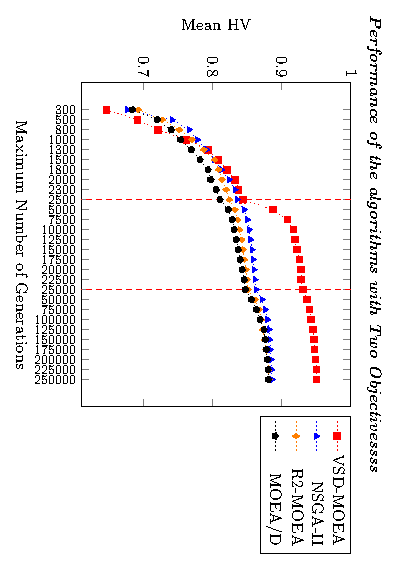
\includegraphics[angle=90,origin=c]{Images/Graphic-Performance-Time_tikz-figure0.eps} \\
\begin{tabular}{l}
 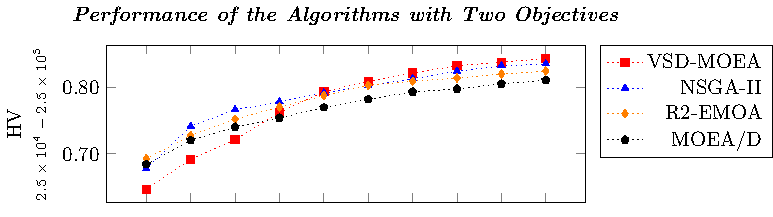
\includegraphics[scale=0.6]{Images/Time_tikz-figure0.eps}\\[0cm]%[-0.14cm] 
 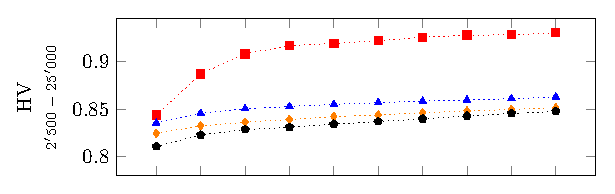
\includegraphics[scale=0.6]{Images/Time_tikz-figure1.eps}\\[0cm]%[-0.18cm]
 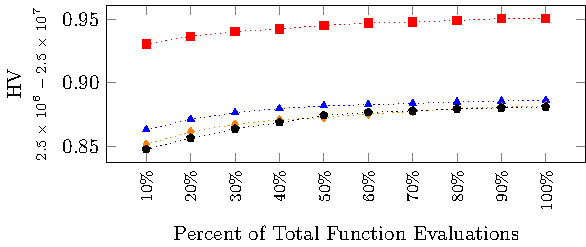
\includegraphics[scale=0.6]{Images/Time_tikz-figure2.eps}
\end{tabular}
%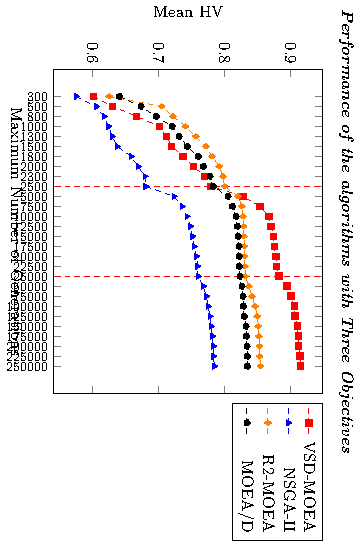
\includegraphics[angle=90,origin=c]{Images/Graphic-Performance-Time_tikz-figure1.pdf} \\
%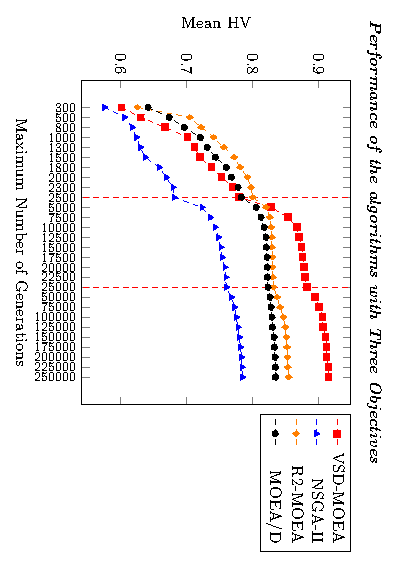
\includegraphics[angle=90,origin=c]{Images/Graphic-Performance-Time_tikz-figure1.eps}
\caption{Performance of the \MOEAS{} considering three ranges of stopping criterion. The configurations take place with short-term (first row), middle-term (second row) and long-term (third row) executions.}\label{fig:Performance_time_2obj}
\end{figure}

\begin{figure}[t]
\centering
%\begin{tikzpicture}[scale=0.8]
\begin{axis}[
title={\textit{\textbf{Performance of \MOEAS{} with Two Objectives}}},
  xlabel= Maximum Number of Generations,
  ylabel=Mean HV,
%  ymin=0.3,
  ymax=1.0,
  xticklabel style = {rotate=90, anchor=east, font=\footnotesize,},
%  label style = {font=\small, },
%xlabel style={yshift=-1cm},
%  xmode=log,
%  log basis x={2},
  legend style=
    {cells={anchor=east},legend pos=outer north east,},
  xticklabels from table={\Performancetimetwo}{mean},xtick=data]
 

\addplot[red,dotted,mark=square*] table [y=VSD_MOEA,x=X]{\Performancetimetwo};
\addlegendentry{VSD-MOEA}

\addplot[blue,dotted,mark=triangle*] table[y= NSGA_II,x=X]{\Performancetimetwo};
\addlegendentry{NSGA-II}
		
\addplot[orange,dotted,mark=diamond*] table [y= R2_MOEA,x=X]{\Performancetimetwo};
\addlegendentry{R2-MOEA}
    
\addplot[black,dotted,mark=pentagon*] table [y= MOEA_D,x=X]{\Performancetimetwo};
\addlegendentry{MOEA/D}
\draw [red, dashed] (axis cs:10, 0) -- (axis cs:10, 1);
\draw [red, dashed] (axis cs:19, 0) -- (axis cs:19, 1);
\end{axis}
\end{tikzpicture}


\begin{tikzpicture}[scale=0.8]
\begin{axis}[
title={\textit{\textbf{Performance of \MOEAS{} with Three Objectives}}},
  xlabel= Maximum Number of Generations,
  ylabel=Mean HV,
%  ymin=0.5,
 % ymax=1.0,
  xticklabel style = {rotate=90, anchor=east, font=\footnotesize,},
  legend style=
    {cells={anchor=east},legend pos=outer north east,},
  xticklabels from table={\Performancetimethree}{mean},xtick=data]

\addplot[red,dashed,mark=square*] table [y=VSD_MOEA,x=X]{\Performancetimethree};
\addlegendentry{VSD-MOEA}

\addplot[blue,dashed,mark=triangle*] table[y= NSGA_II,x=X]{\Performancetimethree};
\addlegendentry{NSGA-II}
		
\addplot[orange,dashed,mark=diamond*] table [y= R2_MOEA,x=X]{\Performancetimethree};
\addlegendentry{R2-MOEA}
    
\addplot[black,dashed,mark=pentagon*] table [y= MOEA_D,x=X]{\Performancetimethree};
\addlegendentry{MOEA/D};
\draw [red, dashed] (axis cs:10, 0) -- (axis cs:10, 1);
\draw [red, dashed] (axis cs:19, 0) -- (axis cs:19, 1);
\end{axis}
\end{tikzpicture}



\caption{Performance of the \MOEAS{} considerin several maximum number of generations.}

%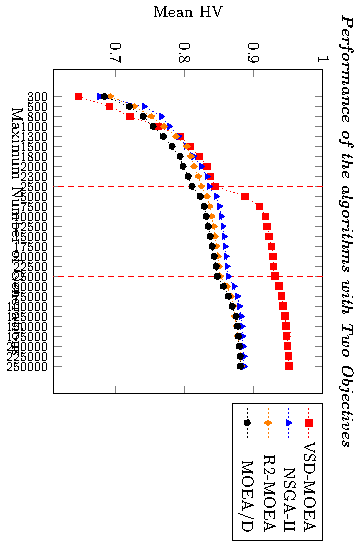
\includegraphics[angle=90,origin=c]{Images/Graphic-Performance-Time_tikz-figure0.pdf} \\
%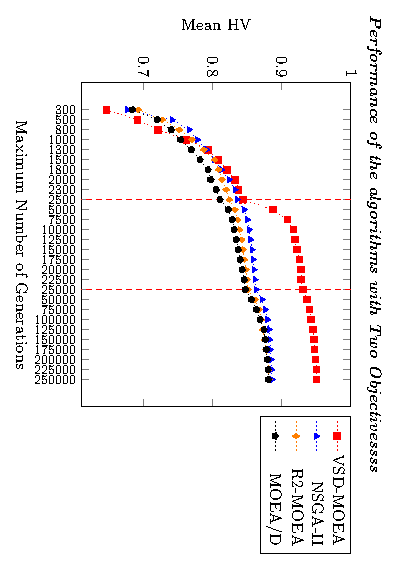
\includegraphics[angle=90,origin=c]{Images/Graphic-Performance-Time_tikz-figure0.eps} \\
\begin{tabular}{l}
 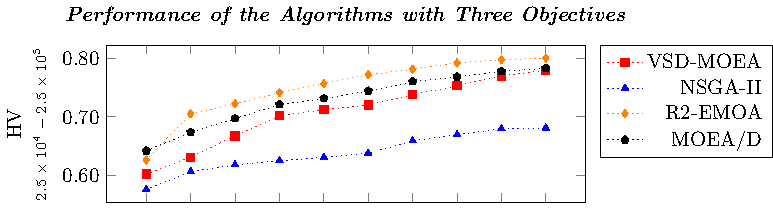
\includegraphics[scale=0.6]{Images/Time_tikz-figure3.eps}\\[0cm]%[-0.14cm] 
 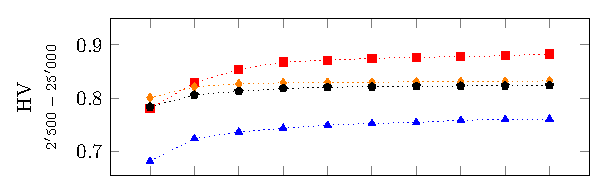
\includegraphics[scale=0.6]{Images/Time_tikz-figure4.eps}\\[0cm]%[-0.18cm]
 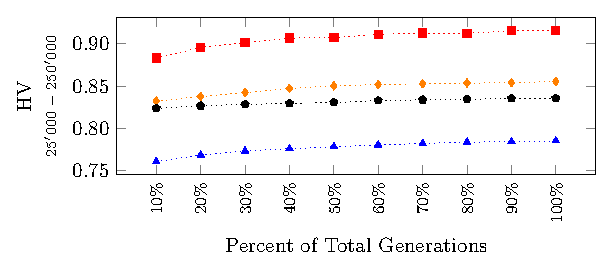
\includegraphics[scale=0.6]{Images/Time_tikz-figure5.eps}
\end{tabular}
\caption{Performance of the \MOEAS{} considering three ranges of stopping criterion. The configurations take place with short-term (first row), middle-term (second row) and long-term (third row) executions.}\label{fig:Performance_time_3obj}
\end{figure}


\subsection{Analysis of the Initial Threshold Value}

One of the disadvantages of including an strategy to control the diversity is that this is usally done at the cost of
incorporating additional parameters in the designed \EA{}.
%
In the case of \VSDMOEA{}, the initial threshold value ($D_I$) must be set.
%
Note that in all the previous experiments $D_I = 0.4$ was used;
%
This value was selected in base of some preliminary experiments.
%
This section is devoted to analyze the performance of \VSDMOEA{} when using different $D_I$ values.
%
Note that, since normalized distances are used, the maximum difference that can appear is $1$.
%
Additionally, note that when $D_I$ is set to 0, no individual is penalized in base of its diversity contribution,
so \VSDMOEA{} would behave as a more traditional \MOEA{}.
%
As a result, the values $D_I = \{0.0, 0.1, 0.2, 0.3, 0.4, 0.5, 0.6, 0.7, 0.8, 0.9\}$ were tested.
%
As in previous experiments, the whole set of benchmark problems were used and
the stopping criterion was set to $250,000$ generations.

Figure \ref{fig:Initial-distance-factor} shows the mean \HV{} ratio attained both for the two-objective and three-objective case.
%
Note that even when setting $D_I = 0$, \VSDMOEA{} attained better \HV{} ratios than other state-of-the-art algorithms.
%
Particularly, such values were $0.912$ and $0.893$ for two and three objectives, respectively.
%
This means that the novel density estimator put forth in this paper is really helpful.
%
However, the increase in performance when using other $D_I$ values is clear.
%
The obtained \HV{} ratio quickly increases as larger $D_I$ values up to $0.4$ are used.
%
Then, with values in the range $[0.5, 0.9]$ the performance decreases slightly.
%
There is quite a large range of values with a really good performance, meaning that 
the behaviour of \VSDMOEA{} is quite robust.
%
Thus, properly setting this parameter is not a complex task.
%

\begin{figure}[t]
\centering
%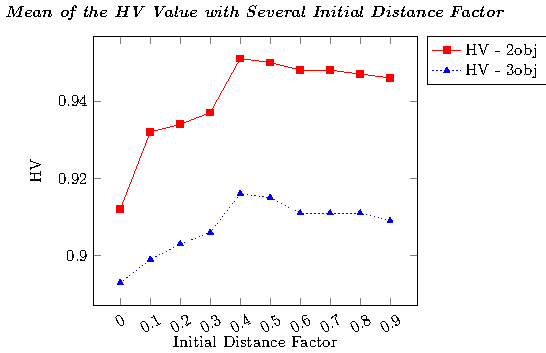
\includegraphics[]{Images/Graphic-Initial-Distance_tikz-figure0.pdf} \\
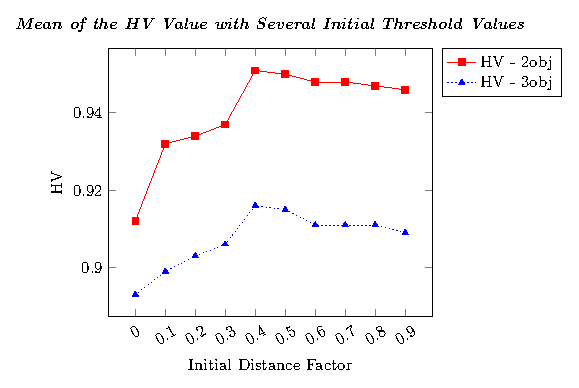
\includegraphics[]{Images/Graphic-Initial-Distance_tikz-figure0.eps} \\
%\begin{tikzpicture}[scale=0.8]
\begin{axis}[
title={\textit{\textbf{Mean of the HV Value with Several Initial Threshold Values}}},
    xlabel=Initial Threshold Value,
  ylabel=HV,
%  xlabel style={yshift=-0.2cm},
  xticklabel style = {rotate=30},
  legend style=
    {cells={anchor=east},legend pos=outer north east,},
  xticklabels from table={\DIHV}{mean},xtick=data]
  
\addplot[red,solid,mark=square*] 
table [y=HV2obj,x=X]{\DIHV};
\addlegendentry{HV - 2obj}
\addplot[blue,dotted,mark=triangle*] table[y= HV3obj,x=X]{\DIHV};
\addlegendentry{HV - 3obj}
		
\end{axis}
\end{tikzpicture}
%%\begin{tikzpicture}[scale=0.8]
%%\begin{axis}[
%%ymin=0.0    ,
%%ymax=0.1,
%%title={\textit{\textbf{Mean of the IGD+ Value with Several Initial Distance Factor}}},
%%    xlabel=Initial Distance Factor,
%%  ylabel=IGD+,
%%  xticklabel style = {rotate=30},
%%  legend style=
%%    {cells={anchor=east},legend pos=outer north east,},
%%  xticklabels from table={\DIIGDP}{mean},xtick=data]
%%\addplot[red,solid,mark=square*] 
%%table [y=IGD2obj,x=X]{\DIIGDP};
%%\addlegendentry{IGD+ 2obj}
%%\addplot[blue,dotted,mark=triangle*] table [y=IGD3obj,x=X]{\DIIGDP};
%%\addlegendentry{IGD+ 3obj}
%%\end{axis}
%%\end{tikzpicture}
%\caption{Mean of Inidicator Considering All Instances with Several Initial Distance Factors}

\caption{Mean of \HV{} values taking into account all instances with several initial threshold values.}\label{fig:Initial-distance-factor}
\end{figure}



%% Please add the following required packages to your document preamble:
% \usepackage{graphicx}
\begin{table*}[t]
\centering
\caption{Statistics IGD+ with two objectives}
\label{tab:StatisticsIGDP_2obj}
%\resizebox{\textwidth}{!}{%
\begin{tabular}{cc|c|c|c|c|c|c|c|c|c|c|c|c|c|c|c}
\cline{2-17}
 & \multicolumn{4}{c|}{\textbf{MOEA/D}} & \multicolumn{4}{c|}{\textbf{NSGA-II}} & \multicolumn{4}{c|}{\textbf{R2-EMOA}} & \multicolumn{4}{c}{\textbf{VSD-MOEA}} \\ \cline{2-17} 
 & \textbf{Min} & \textbf{Max} & \textbf{Mean} & \textbf{Std} & \textbf{Min} & \textbf{Max} & \textbf{Mean} & \textbf{Std} & \textbf{Min} & \textbf{Max} & \textbf{Mean} & \textbf{Std} & \textbf{Min} & \textbf{Max} & \textbf{Mean} & \textbf{Std} \\ \hline
\multicolumn{1}{c|}{\textbf{WFG1}} & 0.006 & 0.015 & 0.008 & 0.002 & 0.006 & 0.014 & 0.008 & 0.002 & 0.006 & 0.061 & 0.013 & 0.014 & 0.006 & 0.019 & 0.008 & 0.003 \\ \hline
\multicolumn{1}{c|}{\textbf{WFG2}} & 0.006 & 0.055 & 0.052 & 0.011 & 0.003 & 0.053 & 0.040 & 0.022 & 0.053 & 0.055 & 0.054 & 0.000 & 0.003 & 0.003 & 0.003 & 0.000 \\ \hline
\multicolumn{1}{c|}{\textbf{WFG3}} & 0.008 & 0.008 & 0.008 & 0.000 & 0.011 & 0.013 & 0.012 & 0.000 & 0.008 & 0.009 & 0.008 & 0.000 & 0.007 & 0.007 & 0.007 & 0.000 \\ \hline
\multicolumn{1}{c|}{\textbf{WFG4}} & 0.007 & 0.007 & 0.007 & 0.000 & 0.007 & 0.010 & 0.008 & 0.001 & 0.005 & 0.005 & 0.005 & 0.000 & 0.006 & 0.006 & 0.006 & 0.000 \\ \hline
\multicolumn{1}{c|}{\textbf{WFG5}} & 0.060 & 0.069 & 0.065 & 0.002 & 0.060 & 0.068 & 0.066 & 0.002 & 0.064 & 0.066 & 0.065 & 0.000 & 0.038 & 0.057 & 0.047 & 0.006 \\ \hline
\multicolumn{1}{c|}{\textbf{WFG6}} & 0.034 & 0.073 & 0.050 & 0.010 & 0.034 & 0.064 & 0.051 & 0.007 & 0.034 & 0.076 & 0.053 & 0.010 & 0.068 & 0.088 & 0.081 & 0.004 \\ \hline
\multicolumn{1}{c|}{\textbf{WFG7}} & 0.007 & 0.007 & 0.007 & 0.000 & 0.008 & 0.010 & 0.009 & 0.000 & 0.005 & 0.006 & 0.005 & 0.000 & 0.006 & 0.006 & 0.006 & 0.000 \\ \hline
\multicolumn{1}{c|}{\textbf{WFG8}} & 0.103 & 0.120 & 0.112 & 0.005 & 0.116 & 0.139 & 0.125 & 0.005 & 0.103 & 0.120 & 0.110 & 0.004 & 0.026 & 0.099 & 0.043 & 0.025 \\ \hline
\multicolumn{1}{c|}{\textbf{WFG9}} & 0.011 & 0.125 & 0.067 & 0.053 & 0.014 & 0.127 & 0.101 & 0.046 & 0.009 & 0.125 & 0.067 & 0.053 & 0.009 & 0.014 & 0.011 & 0.001 \\ \hline
\multicolumn{1}{c|}{\textbf{DTLZ1}} & 0.001 & 0.001 & 0.001 & 0.000 & 0.002 & 0.002 & 0.002 & 0.000 & 0.001 & 0.001 & 0.001 & 0.000 & 0.001 & 0.001 & 0.001 & 0.000 \\ \hline
\multicolumn{1}{c|}{\textbf{DTLZ2}} & 0.002 & 0.002 & 0.002 & 0.000 & 0.002 & 0.003 & 0.003 & 0.000 & 0.002 & 0.002 & 0.002 & 0.000 & 0.002 & 0.002 & 0.002 & 0.000 \\ \hline
\multicolumn{1}{c|}{\textbf{DTLZ3}} & 0.002 & 0.002 & 0.002 & 0.000 & 0.002 & 0.003 & 0.002 & 0.000 & 0.002 & 0.002 & 0.002 & 0.000 & 0.002 & 0.002 & 0.002 & 0.000 \\ \hline
\multicolumn{1}{c|}{\textbf{DTLZ4}} & 0.002 & 0.363 & 0.105 & 0.163 & 0.002 & 0.363 & 0.064 & 0.136 & 0.002 & 0.363 & 0.167 & 0.180 & 0.002 & 0.002 & 0.002 & 0.000 \\ \hline
\multicolumn{1}{c|}{\textbf{DTLZ5}} & 0.002 & 0.002 & 0.002 & 0.000 & 0.002 & 0.003 & 0.003 & 0.000 & 0.002 & 0.002 & 0.002 & 0.000 & 0.002 & 0.002 & 0.002 & 0.000 \\ \hline
\multicolumn{1}{c|}{\textbf{DTLZ6}} & 0.022 & 0.149 & 0.076 & 0.027 & 0.126 & 0.315 & 0.205 & 0.036 & 0.019 & 0.128 & 0.078 & 0.027 & 0.002 & 0.002 & 0.002 & 0.000 \\ \hline
\multicolumn{1}{c|}{\textbf{DTLZ7}} & 0.003 & 0.003 & 0.003 & 0.000 & 0.002 & 0.003 & 0.003 & 0.000 & 0.002 & 0.002 & 0.002 & 0.000 & 0.003 & 0.003 & 0.003 & 0.000 \\ \hline
\multicolumn{1}{c|}{\textbf{UF1}} & 0.004 & 0.004 & 0.004 & 0.000 & 0.005 & 0.006 & 0.006 & 0.000 & 0.003 & 0.005 & 0.004 & 0.001 & 0.003 & 0.003 & 0.003 & 0.000 \\ \hline
\multicolumn{1}{c|}{\textbf{UF2}} & 0.003 & 0.005 & 0.004 & 0.000 & 0.008 & 0.010 & 0.010 & 0.000 & 0.004 & 0.006 & 0.005 & 0.001 & 0.004 & 0.007 & 0.005 & 0.001 \\ \hline
\multicolumn{1}{c|}{\textbf{UF3}} & 0.141 & 0.237 & 0.180 & 0.022 & 0.052 & 0.127 & 0.084 & 0.020 & 0.119 & 0.210 & 0.183 & 0.021 & 0.038 & 0.095 & 0.057 & 0.013 \\ \hline
\multicolumn{1}{c|}{\textbf{UF4}} & 0.024 & 0.031 & 0.026 & 0.001 & 0.027 & 0.039 & 0.033 & 0.003 & 0.019 & 0.023 & 0.021 & 0.001 & 0.020 & 0.024 & 0.022 & 0.001 \\ \hline
\multicolumn{1}{c|}{\textbf{UF5}} & 0.079 & 0.593 & 0.265 & 0.120 & 0.091 & 0.254 & 0.142 & 0.033 & 0.079 & 0.521 & 0.215 & 0.131 & 0.088 & 0.154 & 0.132 & 0.014 \\ \hline
\multicolumn{1}{c|}{\textbf{UF6}} & 0.066 & 0.529 & 0.380 & 0.108 & 0.037 & 0.542 & 0.193 & 0.114 & 0.064 & 0.432 & 0.266 & 0.103 & 0.021 & 0.065 & 0.038 & 0.011 \\ \hline
\multicolumn{1}{c|}{\textbf{UF7}} & 0.003 & 0.005 & 0.004 & 0.000 & 0.007 & 0.008 & 0.007 & 0.000 & 0.003 & 0.242 & 0.046 & 0.082 & 0.003 & 0.009 & 0.004 & 0.001 \\ \hline
\multicolumn{1}{c|}{\textbf{Mean}} & 0.026 & 0.105 & 0.062 & 0.023 & 0.027 & 0.095 & 0.051 & 0.019 & 0.026 & 0.107 & 0.060 & 0.027 & 0.016 & 0.029 & 0.021 & 0.003 \\ \hline
\end{tabular}%
%}
\end{table*}



%%% Please add the following required packages to your document preamble:
%%% \usepackage{graphicx}
%%
%%\begin{table*}[t]
%%\caption{Statistics IGD+ with two objectives}
%%\label{tab:StatisticsIGDP_2obj}
%%%\resizebox{\textwidth}{!}{%
%%\begin{tabular}{c|c|c|c|c|c|c|c|c|c|c|c|c|c|c|c|c|}
%%\cline{2-17}
%% & \multicolumn{4}{c|}{\textbf{MOEA/D}} & \multicolumn{4}{c|}{\textbf{NSGA-II}} & \multicolumn{4}{c|}{\textbf{R2-MOEA}} & \multicolumn{4}{c|}{\textbf{VSD-MOEA}} \\ \cline{2-17} 
%% & \textbf{Min} & \textbf{Max} & \textbf{Mean} & \textbf{Std} & \textbf{Min} & \textbf{Max} & \textbf{Mean} & \textbf{Std} & \textbf{Min} & \textbf{Max} & \textbf{Mean} & \textbf{Std} & \textbf{Min} & \textbf{Max} & \textbf{Mean} & \textbf{Std} \\ \hline
%%\multicolumn{1}{|c|}{\textbf{WFG1}} & 0.006 & 0.015 & 0.008 & 0.002 & 0.006 & 0.014 & 0.008 & 0.002 & 0.006 & 0.061 & 0.013 & 0.014 & 0.006 & 0.025 & 0.007 & 0.003 \\ \hline
%%\multicolumn{1}{|c|}{\textbf{WFG2}} & 0.006 & 0.055 & 0.052 & 0.011 & 0.003 & 0.053 & 0.040 & 0.022 & 0.053 & 0.055 & 0.054 & 0.000 & 0.003 & 0.003 & 0.003 & 0.000 \\ \hline
%%\multicolumn{1}{|c|}{\textbf{WFG3}} & 0.008 & 0.008 & 0.008 & 0.000 & 0.011 & 0.013 & 0.012 & 0.000 & 0.008 & 0.009 & 0.008 & 0.000 & 0.007 & 0.007 & 0.007 & 0.000 \\ \hline
%%\multicolumn{1}{|c|}{\textbf{WFG4}} & 0.007 & 0.007 & 0.007 & 0.000 & 0.007 & 0.010 & 0.008 & 0.001 & 0.005 & 0.005 & 0.005 & 0.000 & 0.006 & 0.006 & 0.006 & 0.000 \\ \hline
%%\multicolumn{1}{|c|}{\textbf{WFG5}} & 0.060 & 0.069 & 0.065 & 0.002 & 0.060 & 0.068 & 0.066 & 0.002 & 0.064 & 0.066 & 0.065 & 0.000 & 0.033 & 0.053 & 0.040 & 0.005 \\ \hline
%%\multicolumn{1}{|c|}{\textbf{WFG6}} & 0.034 & 0.073 & 0.050 & 0.010 & 0.034 & 0.064 & 0.051 & 0.007 & 0.034 & 0.076 & 0.053 & 0.010 & 0.068 & 0.090 & 0.081 & 0.005 \\ \hline
%%\multicolumn{1}{|c|}{\textbf{WFG7}} & 0.007 & 0.007 & 0.007 & 0.000 & 0.008 & 0.010 & 0.009 & 0.000 & 0.005 & 0.006 & 0.005 & 0.000 & 0.006 & 0.006 & 0.006 & 0.000 \\ \hline
%%\multicolumn{1}{|c|}{\textbf{WFG8}} & 0.103 & 0.120 & 0.112 & 0.005 & 0.116 & 0.139 & 0.125 & 0.005 & 0.103 & 0.120 & 0.110 & 0.004 & 0.024 & 0.035 & 0.029 & 0.003 \\ \hline
%%\multicolumn{1}{|c|}{\textbf{WFG9}} & 0.011 & 0.125 & 0.067 & 0.053 & 0.014 & 0.127 & 0.101 & 0.046 & 0.009 & 0.125 & 0.067 & 0.053 & 0.009 & 0.015 & 0.011 & 0.001 \\ \hline
%%\multicolumn{1}{|c|}{\textbf{DTLZ1}} & 0.001 & 0.001 & 0.001 & 0.000 & 0.002 & 0.002 & 0.002 & 0.000 & 0.001 & 0.001 & 0.001 & 0.000 & 0.001 & 0.001 & 0.001 & 0.000 \\ \hline
%%\multicolumn{1}{|c|}{\textbf{DTLZ2}} & 0.002 & 0.002 & 0.002 & 0.000 & 0.002 & 0.003 & 0.003 & 0.000 & 0.002 & 0.002 & 0.002 & 0.000 & 0.002 & 0.002 & 0.002 & 0.000 \\ \hline
%%\multicolumn{1}{|c|}{\textbf{DTLZ3}} & 0.002 & 0.002 & 0.002 & 0.000 & 0.002 & 0.003 & 0.002 & 0.000 & 0.002 & 0.002 & 0.002 & 0.000 & 0.002 & 0.002 & 0.002 & 0.000 \\ \hline
%%\multicolumn{1}{|c|}{\textbf{DTLZ4}} & 0.002 & 0.363 & 0.105 & 0.163 & 0.002 & 0.363 & 0.064 & 0.136 & 0.002 & 0.363 & 0.167 & 0.180 & 0.002 & 0.002 & 0.002 & 0.000 \\ \hline
%%\multicolumn{1}{|c|}{\textbf{DTLZ5}} & 0.002 & 0.002 & 0.002 & 0.000 & 0.002 & 0.003 & 0.003 & 0.000 & 0.002 & 0.002 & 0.002 & 0.000 & 0.002 & 0.002 & 0.002 & 0.000 \\ \hline
%%\multicolumn{1}{|c|}{\textbf{DTLZ6}} & 0.022 & 0.149 & 0.076 & 0.027 & 0.126 & 0.315 & 0.205 & 0.036 & 0.019 & 0.128 & 0.078 & 0.027 & 0.002 & 0.002 & 0.002 & 0.000 \\ \hline
%%\multicolumn{1}{|c|}{\textbf{DTLZ7}} & 0.003 & 0.003 & 0.003 & 0.000 & 0.002 & 0.003 & 0.003 & 0.000 & 0.002 & 0.002 & 0.002 & 0.000 & 0.003 & 0.003 & 0.003 & 0.000 \\ \hline
%%\multicolumn{1}{|c|}{\textbf{UF1}} & 0.004 & 0.004 & 0.004 & 0.000 & 0.005 & 0.006 & 0.006 & 0.000 & 0.003 & 0.005 & 0.004 & 0.001 & 0.003 & 0.003 & 0.003 & 0.000 \\ \hline
%%\multicolumn{1}{|c|}{\textbf{UF2}} & 0.003 & 0.005 & 0.004 & 0.000 & 0.008 & 0.010 & 0.010 & 0.000 & 0.004 & 0.006 & 0.005 & 0.001 & 0.005 & 0.008 & 0.006 & 0.001 \\ \hline
%%\multicolumn{1}{|c|}{\textbf{UF3}} & 0.141 & 0.237 & 0.180 & 0.022 & 0.052 & 0.127 & 0.084 & 0.020 & 0.119 & 0.210 & 0.183 & 0.021 & 0.043 & 0.077 & 0.052 & 0.006 \\ \hline
%%\multicolumn{1}{|c|}{\textbf{UF4}} & 0.024 & 0.031 & 0.026 & 0.001 & 0.027 & 0.039 & 0.033 & 0.003 & 0.019 & 0.023 & 0.021 & 0.001 & 0.021 & 0.024 & 0.022 & 0.001 \\ \hline
%%\multicolumn{1}{|c|}{\textbf{UF5}} & 0.079 & 0.593 & 0.265 & 0.120 & 0.091 & 0.254 & 0.142 & 0.033 & 0.079 & 0.521 & 0.215 & 0.131 & 0.083 & 0.145 & 0.118 & 0.015 \\ \hline
%%\multicolumn{1}{|c|}{\textbf{UF6}} & 0.066 & 0.529 & 0.380 & 0.108 & 0.037 & 0.542 & 0.193 & 0.114 & 0.064 & 0.432 & 0.266 & 0.103 & 0.019 & 0.034 & 0.026 & 0.005 \\ \hline
%%\multicolumn{1}{|c|}{\textbf{UF7}} & 0.003 & 0.005 & 0.004 & 0.000 & 0.007 & 0.008 & 0.007 & 0.000 & 0.003 & 0.242 & 0.046 & 0.082 & 0.003 & 0.005 & 0.004 & 0.000 \\ \hline
%%\multicolumn{1}{|c|}{\textbf{Mean}} & \textbf{0.026} & \textbf{0.105} & \textbf{0.062} & \textbf{0.023} & \textbf{0.027} & \textbf{0.095} & \textbf{0.051} & \textbf{0.019} & \textbf{0.026} & \textbf{0.107} & \textbf{0.060} & \textbf{0.027} & \textbf{0.015} & \textbf{0.024} & \textbf{0.019} & \textbf{0.002} \\ \hline
%%\end{tabular}%
%%%}
%%\end{table*}
%%

%% Please add the following required packages to your document preamble:
% \usepackage{graphicx}
\begin{table*}[t]
\caption{Summary of the IGD+ results attained for problems with three objectives}
\label{tab:StatisticsIGDP_3obj}
\centering
%\resizebox{\textwidth}{!}{%
\begin{tabular}{cc|c|c|c|c|c|c|c|c|c|c|c|c|c|c|c}
\cline{2-17}
\textbf{}                           & \multicolumn{4}{c|}{\textbf{MOEA/D}}                       & \multicolumn{4}{c|}{\textbf{NSGA-II}}                      & \multicolumn{4}{c|}{\textbf{R2-EMOA}}                             & \multicolumn{4}{c}{\textbf{VSD-MOEA}}                            \\ \cline{2-17} 
                                    & \textbf{Min} & \textbf{Max} & \textbf{Mean} & \textbf{Std} & \textbf{Min} & \textbf{Max} & \textbf{Mean} & \textbf{Std} & \textbf{Min}   & \textbf{Max}   & \textbf{Mean}  & \textbf{Std}   & \textbf{Min}   & \textbf{Max}   & \textbf{Mean}  & \textbf{Std}   \\ \hline
\multicolumn{1}{c|}{\textbf{WFG1}}  & 0.080        & 0.100        & 0.090         & 0.005        & 0.142        & 0.179        & 0.160         & 0.010        & 0.058          & 0.098          & 0.079          & 0.010          & \textbf{0.049} & \textbf{0.070} & \textbf{0.058} & \textbf{0.006} \\ \hline
\multicolumn{1}{c|}{\textbf{WFG2}}  & 0.057        & 0.068        & 0.063         & 0.002        & 0.073        & 0.133        & 0.097         & 0.014        & 0.102          & 0.104          & 0.103          & 0.000          & \textbf{0.031} & \textbf{0.048} & \textbf{0.037} & \textbf{0.004} \\ \hline
\multicolumn{1}{c|}{\textbf{WFG3}}  & 0.023        & 0.023        & 0.023         & 0.000        & 0.031        & 0.061        & 0.039         & 0.005        & \textbf{0.022} & \textbf{0.023} & \textbf{0.022} & \textbf{0.000} & 0.033          & 0.033          & 0.033          & 0.000          \\ \hline
\multicolumn{1}{c|}{\textbf{WFG4}}  & 0.127        & 0.127        & 0.127         & 0.000        & 0.121        & 0.144        & 0.132         & 0.005        & 0.095          & 0.098          & 0.097          & 0.001          & \textbf{0.090} & \textbf{0.094} & \textbf{0.093} & \textbf{0.001} \\ \hline
\multicolumn{1}{c|}{\textbf{WFG5}}  & 0.177        & 0.184        & 0.181         & 0.002        & 0.160        & 0.186        & 0.170         & 0.005        & 0.147          & 0.158          & 0.153          & 0.003          & \textbf{0.140} & \textbf{0.150} & \textbf{0.146} & \textbf{0.003} \\ \hline
\multicolumn{1}{c|}{\textbf{WFG6}}  & 0.155        & 0.205        & 0.175         & 0.012        & 0.159        & 0.196        & 0.177         & 0.009        & \textbf{0.122} & \textbf{0.151} & \textbf{0.140} & \textbf{0.007} & 0.156          & 0.173          & 0.166          & 0.005          \\ \hline
\multicolumn{1}{c|}{\textbf{WFG7}}  & 0.127        & 0.127        & 0.127         & 0.000        & 0.113        & 0.138        & 0.123         & 0.007        & 0.094          & 0.102          & 0.097          & 0.001          & \textbf{0.092} & \textbf{0.094} & \textbf{0.094} & \textbf{0.001} \\ \hline
\multicolumn{1}{c|}{\textbf{WFG8}}  & 0.189        & 0.194        & 0.192         & 0.001        & 0.244        & 0.274        & 0.256         & 0.008        & 0.161          & 0.166          & 0.163          & 0.001          & \textbf{0.099} & \textbf{0.154} & \textbf{0.109} & \textbf{0.015} \\ \hline
\multicolumn{1}{c|}{\textbf{WFG9}}  & 0.130        & 0.240        & 0.154         & 0.036        & 0.138        & 0.246        & 0.224         & 0.025        & 0.099          & 0.211          & 0.119          & 0.037          & \textbf{0.099} & \textbf{0.210} & \textbf{0.118} & \textbf{0.036} \\ \hline
\multicolumn{1}{c|}{\textbf{DTLZ1}} & 0.014        & 0.014        & 0.014         & 0.000        & 0.017        & 0.020        & 0.018         & 0.001        & \textbf{0.013} & \textbf{0.014} & \textbf{0.014} & \textbf{0.000} & 0.014          & 0.014          & 0.014          & 0.000          \\ \hline
\multicolumn{1}{c|}{\textbf{DTLZ2}} & 0.027        & 0.027        & 0.027         & 0.000        & 0.030        & 0.036        & 0.032         & 0.001        & \textbf{0.023} & \textbf{0.024} & \textbf{0.023} & \textbf{0.000} & 0.024          & 0.025          & 0.024          & 0.000          \\ \hline
\multicolumn{1}{c|}{\textbf{DTLZ3}} & 0.027        & 0.027        & 0.027         & 0.000        & 0.027        & 0.032        & 0.030         & 0.001        & \textbf{0.023} & \textbf{0.023} & \textbf{0.023} & \textbf{0.000} & 0.024          & 0.025          & 0.024          & 0.000          \\ \hline
\multicolumn{1}{c|}{\textbf{DTLZ4}} & 0.027        & 0.595        & 0.092         & 0.181        & 0.028        & 0.036        & 0.032         & 0.001        & 0.023          & 0.595          & 0.190          & 0.225          & \textbf{0.024} & \textbf{0.025} & \textbf{0.024} & \textbf{0.000} \\ \hline
\multicolumn{1}{c|}{\textbf{DTLZ5}} & 0.003        & 0.003        & 0.003         & 0.000        & 0.003        & 0.003        & 0.003         & 0.000        & 0.002          & 0.002          & 0.002          & 0.000          & \textbf{0.002} & \textbf{0.002} & \textbf{0.002} & \textbf{0.000} \\ \hline
\multicolumn{1}{c|}{\textbf{DTLZ6}} & 0.022        & 0.163        & 0.087         & 0.032        & 0.126        & 0.224        & 0.187         & 0.027        & 0.003          & 0.136          & 0.069          & 0.033          & \textbf{0.002} & \textbf{0.002} & \textbf{0.002} & \textbf{0.000} \\ \hline
\multicolumn{1}{c|}{\textbf{DTLZ7}} & 0.045        & 0.045        & 0.045         & 0.000        & 0.038        & 0.052        & 0.044         & 0.003        & 0.060          & 0.087          & 0.079          & 0.008          & \textbf{0.027} & \textbf{0.029} & \textbf{0.028} & \textbf{0.000} \\ \hline
\multicolumn{1}{c|}{\textbf{UF8}}   & 0.048        & 0.365        & 0.069         & 0.051        & 0.093        & 0.220        & 0.178         & 0.031        & 0.027          & 0.159          & 0.033          & 0.022          & \textbf{0.025} & \textbf{0.034} & \textbf{0.029} & \textbf{0.002} \\ \hline
\multicolumn{1}{c|}{\textbf{UF9}}   & 0.041        & 0.151        & 0.086         & 0.049        & 0.106        & 0.314        & 0.139         & 0.049        & 0.025          & 0.137          & 0.094          & 0.053          & \textbf{0.022} & \textbf{0.028} & \textbf{0.024} & \textbf{0.001} \\ \hline
\multicolumn{1}{c|}{\textbf{UF10}}  & 0.163        & 0.565        & 0.294         & 0.125        & 0.198        & 0.658        & 0.261         & 0.080        & 0.159          & 0.553          & 0.257          & 0.131          & \textbf{0.070} & \textbf{0.187} & \textbf{0.103} & \textbf{0.026} \\ \hline
\multicolumn{1}{c|}{\textbf{Mean}}  & 0.078        & 0.170        & 0.099         & 0.026        & 0.097        & 0.166        & 0.121         & 0.015        & 0.066          & 0.150          & 0.093          & 0.028          & 0.054          & 0.074          & 0.059          & 0.005          \\ \hline
\end{tabular}%
%}
\end{table*}

%% Please add the following required packages to your document preamble:
%% \usepackage{graphicx}
%\begin{table*}[t]
%\caption{Statistics IGD+ with three objectives}
%\label{tab:StatisticsIGDP_3obj}
%%\resizebox{\textwidth}{!}{%
%\begin{tabular}{c|c|c|c|c|c|c|c|c|c|c|c|c|c|c|c|c|}
%\cline{2-17}
% & \multicolumn{4}{c|}{\textbf{MOEA/D}} & \multicolumn{4}{c|}{\textbf{NSGA-II}} & \multicolumn{4}{c|}{\textbf{R2-MOEA}} & \multicolumn{4}{c|}{\textbf{VSD-MOEA}} \\ \cline{2-17} 
% & \textbf{Min} & \textbf{Max} & \textbf{Mean} & \textbf{Std} & \textbf{Min} & \textbf{Max} & \textbf{Mean} & \textbf{Std} & \textbf{Min} & \textbf{Max} & \textbf{Mean} & \textbf{Std} & \textbf{Min} & \textbf{Max} & \textbf{Mean} & \textbf{Std} \\ \hline
%\multicolumn{1}{|c|}{\textbf{WFG1}} & 0.080 & 0.100 & 0.090 & 0.005 & 0.142 & 0.179 & 0.160 & 0.010 & 0.058 & 0.098 & 0.079 & 0.010 & 0.050 & 0.066 & 0.056 & 0.004 \\ \hline
%\multicolumn{1}{|c|}{\textbf{WFG2}} & 0.057 & 0.068 & 0.063 & 0.002 & 0.073 & 0.133 & 0.097 & 0.014 & 0.102 & 0.104 & 0.103 & 0.000 & 0.031 & 0.044 & 0.038 & 0.003 \\ \hline
%\multicolumn{1}{|c|}{\textbf{WFG3}} & 0.023 & 0.023 & 0.023 & 0.000 & 0.031 & 0.061 & 0.039 & 0.005 & 0.022 & 0.023 & 0.022 & 0.000 & 0.033 & 0.033 & 0.033 & 0.000 \\ \hline
%\multicolumn{1}{|c|}{\textbf{WFG4}} & 0.127 & 0.127 & 0.127 & 0.000 & 0.121 & 0.144 & 0.132 & 0.005 & 0.095 & 0.098 & 0.097 & 0.001 & 0.091 & 0.094 & 0.093 & 0.001 \\ \hline
%\multicolumn{1}{|c|}{\textbf{WFG5}} & 0.177 & 0.184 & 0.181 & 0.002 & 0.160 & 0.186 & 0.170 & 0.005 & 0.147 & 0.158 & 0.153 & 0.003 & 0.143 & 0.155 & 0.147 & 0.002 \\ \hline
%\multicolumn{1}{|c|}{\textbf{WFG6}} & 0.155 & 0.205 & 0.175 & 0.012 & 0.159 & 0.196 & 0.177 & 0.009 & 0.122 & 0.151 & 0.140 & 0.007 & 0.143 & 0.173 & 0.163 & 0.008 \\ \hline
%\multicolumn{1}{|c|}{\textbf{WFG7}} & 0.127 & 0.127 & 0.127 & 0.000 & 0.113 & 0.138 & 0.123 & 0.007 & 0.094 & 0.102 & 0.097 & 0.001 & 0.092 & 0.094 & 0.093 & 0.001 \\ \hline
%\multicolumn{1}{|c|}{\textbf{WFG8}} & 0.189 & 0.194 & 0.192 & 0.001 & 0.244 & 0.274 & 0.256 & 0.008 & 0.161 & 0.166 & 0.163 & 0.001 & 0.101 & 0.121 & 0.106 & 0.005 \\ \hline
%\multicolumn{1}{|c|}{\textbf{WFG9}} & 0.130 & 0.240 & 0.154 & 0.036 & 0.138 & 0.246 & 0.224 & 0.025 & 0.099 & 0.211 & 0.119 & 0.037 & 0.101 & 0.162 & 0.106 & 0.010 \\ \hline
%\multicolumn{1}{|c|}{\textbf{DTLZ1}} & 0.014 & 0.014 & 0.014 & 0.000 & 0.017 & 0.020 & 0.018 & 0.001 & 0.013 & 0.014 & 0.014 & 0.000 & 0.014 & 0.014 & 0.014 & 0.000 \\ \hline
%\multicolumn{1}{|c|}{\textbf{DTLZ2}} & 0.027 & 0.027 & 0.027 & 0.000 & 0.030 & 0.036 & 0.032 & 0.001 & 0.023 & 0.024 & 0.023 & 0.000 & 0.024 & 0.025 & 0.024 & 0.000 \\ \hline
%\multicolumn{1}{|c|}{\textbf{DTLZ3}} & 0.027 & 0.027 & 0.027 & 0.000 & 0.027 & 0.032 & 0.030 & 0.001 & 0.023 & 0.023 & 0.023 & 0.000 & 0.024 & 0.025 & 0.024 & 0.000 \\ \hline
%\multicolumn{1}{|c|}{\textbf{DTLZ4}} & 0.027 & 0.595 & 0.092 & 0.181 & 0.028 & 0.036 & 0.032 & 0.001 & 0.023 & 0.595 & 0.190 & 0.225 & 0.024 & 0.025 & 0.024 & 0.000 \\ \hline
%\multicolumn{1}{|c|}{\textbf{DTLZ5}} & 0.003 & 0.003 & 0.003 & 0.000 & 0.003 & 0.003 & 0.003 & 0.000 & 0.002 & 0.002 & 0.002 & 0.000 & 0.002 & 0.002 & 0.002 & 0.000 \\ \hline
%\multicolumn{1}{|c|}{\textbf{DTLZ6}} & 0.022 & 0.163 & 0.087 & 0.032 & 0.126 & 0.224 & 0.187 & 0.027 & 0.003 & 0.136 & 0.069 & 0.033 & 0.002 & 0.002 & 0.002 & 0.000 \\ \hline
%\multicolumn{1}{|c|}{\textbf{DTLZ7}} & 0.045 & 0.045 & 0.045 & 0.000 & 0.038 & 0.052 & 0.044 & 0.003 & 0.060 & 0.087 & 0.079 & 0.008 & 0.027 & 0.029 & 0.028 & 0.000 \\ \hline
%\multicolumn{1}{|c|}{\textbf{UF8}} & 0.048 & 0.365 & 0.069 & 0.051 & 0.093 & 0.220 & 0.178 & 0.031 & 0.027 & 0.159 & 0.033 & 0.022 & 0.026 & 0.034 & 0.029 & 0.002 \\ \hline
%\multicolumn{1}{|c|}{\textbf{UF9}} & 0.041 & 0.151 & 0.086 & 0.049 & 0.106 & 0.314 & 0.139 & 0.049 & 0.025 & 0.137 & 0.094 & 0.053 & 0.022 & 0.030 & 0.025 & 0.002 \\ \hline
%\multicolumn{1}{|c|}{\textbf{UF10}} & 0.163 & 0.565 & 0.294 & 0.125 & 0.198 & 0.658 & 0.261 & 0.080 & 0.159 & 0.553 & 0.257 & 0.131 & 0.061 & 0.168 & 0.099 & 0.026 \\ \hline
%\multicolumn{1}{|c|}{\textbf{Mean}} & \textbf{0.078} & \textbf{0.170} & \textbf{0.099} & \textbf{0.026} & \textbf{0.097} & \textbf{0.166} & \textbf{0.121} & \textbf{0.015} & \textbf{0.066} & \textbf{0.150} & \textbf{0.093} & \textbf{0.028} & \textbf{0.053} & \textbf{0.068} & \textbf{0.058} & \textbf{0.003} \\ \hline
%\end{tabular}%
%%}
%\end{table*}

%%% Please add the following required packages to your document preamble:
%% \usepackage{graphicx}
%\begin{table*}[t]
%\caption{Statistical Tests of IGD+ with Two Objectives}
%\label{tab:Tests_IGDP_2obj}
%\centering
%%\resizebox{\textwidth}{!}{%
%\begin{tabular}{c|c|c|c|c|c|c|c|c|c|c|c|c|c|c|c|c|}
%\cline{2-17}
%\textbf{} & \multicolumn{4}{c|}{\textbf{MOEA/D}} & \multicolumn{4}{c|}{\textbf{NSGA-II}} & \multicolumn{4}{c|}{\textbf{R2-MOEA}} & \multicolumn{4}{c|}{\textbf{VSD-MOEA}} \\ \cline{2-17} 
% & \textbf{$\uparrow$} & \textbf{$\downarrow$} & \textbf{$\leftrightarrow$} & \textbf{Diff} & \textbf{$\uparrow$} & \textbf{$\downarrow$} & \textbf{$\leftrightarrow$} & \textbf{Diff} & \textbf{$\uparrow$} & \textbf{$\downarrow$} & \textbf{$\leftrightarrow$} & \textbf{Diff} & \textbf{$\uparrow$} & \textbf{$\downarrow$} & \textbf{$\leftrightarrow$} & \textbf{Diff} \\ \hline
%\multicolumn{1}{|c|}{\textbf{WFG1}} & 1 & 1 & 1 & 0.000 & 0 & 1 & 2 & 0.001 & 0 & 2 & 1 & 0.006 & 3 & 0 & 0 & 0.000 \\ \hline
%\multicolumn{1}{|c|}{\textbf{WFG2}} & 1 & 2 & 0 & 0.049 & 2 & 1 & 0 & 0.037 & 0 & 3 & 0 & 0.051 & 3 & 0 & 0 & 0.000 \\ \hline
%\multicolumn{1}{|c|}{\textbf{WFG3}} & 2 & 1 & 0 & 0.000 & 0 & 3 & 0 & 0.005 & 1 & 2 & 0 & 0.001 & 3 & 0 & 0 & 0.000 \\ \hline
%\multicolumn{1}{|c|}{\textbf{WFG4}} & 1 & 2 & 0 & 0.001 & 0 & 3 & 0 & 0.003 & 3 & 0 & 0 & 0.000 & 2 & 1 & 0 & 0.001 \\ \hline
%\multicolumn{1}{|c|}{\textbf{WFG5}} & 0 & 1 & 2 & 0.026 & 0 & 2 & 1 & 0.026 & 1 & 1 & 1 & 0.025 & 3 & 0 & 0 & 0.000 \\ \hline
%\multicolumn{1}{|c|}{\textbf{WFG6}} & 1 & 0 & 2 & 0.000 & 1 & 0 & 2 & 0.001 & 1 & 0 & 2 & 0.002 & 0 & 3 & 0 & 0.030 \\ \hline
%\multicolumn{1}{|c|}{\textbf{WFG7}} & 1 & 2 & 0 & 0.001 & 0 & 3 & 0 & 0.003 & 3 & 0 & 0 & 0.000 & 2 & 1 & 0 & 0.001 \\ \hline
%\multicolumn{1}{|c|}{\textbf{WFG8}} & 1 & 1 & 1 & 0.083 & 0 & 3 & 0 & 0.096 & 1 & 1 & 1 & 0.082 & 3 & 0 & 0 & 0.000 \\ \hline
%\multicolumn{1}{|c|}{\textbf{WFG9}} & 1 & 1 & 1 & 0.056 & 0 & 3 & 0 & 0.090 & 1 & 1 & 1 & 0.055 & 3 & 0 & 0 & 0.000 \\ \hline
%\multicolumn{1}{|c|}{\textbf{DTLZ1}} & 3 & 0 & 0 & 0.000 & 0 & 3 & 0 & 0.000 & 1 & 1 & 1 & 0.000 & 1 & 1 & 1 & 0.000 \\ \hline
%\multicolumn{1}{|c|}{\textbf{DTLZ2}} & 1 & 2 & 0 & 0.000 & 0 & 3 & 0 & 0.001 & 3 & 0 & 0 & 0.000 & 2 & 1 & 0 & 0.000 \\ \hline
%\multicolumn{1}{|c|}{\textbf{DTLZ3}} & 1 & 2 & 0 & 0.000 & 0 & 3 & 0 & 0.001 & 3 & 0 & 0 & 0.000 & 2 & 1 & 0 & 0.000 \\ \hline
%\multicolumn{1}{|c|}{\textbf{DTLZ4}} & 0 & 2 & 1 & 0.103 & 1 & 1 & 1 & 0.062 & 0 & 0 & 3 & 0.165 & 2 & 0 & 1 & 0.000 \\ \hline
%\multicolumn{1}{|c|}{\textbf{DTLZ5}} & 1 & 2 & 0 & 0.000 & 0 & 3 & 0 & 0.001 & 3 & 0 & 0 & 0.000 & 2 & 1 & 0 & 0.000 \\ \hline
%\multicolumn{1}{|c|}{\textbf{DTLZ6}} & 1 & 1 & 1 & 0.073 & 0 & 3 & 0 & 0.203 & 1 & 1 & 1 & 0.076 & 3 & 0 & 0 & 0.000 \\ \hline
%\multicolumn{1}{|c|}{\textbf{DTLZ7}} & 0 & 3 & 0 & 0.001 & 1 & 1 & 1 & 0.001 & 3 & 0 & 0 & 0.000 & 1 & 1 & 1 & 0.001 \\ \hline
%\multicolumn{1}{|c|}{\textbf{UF1}} & 1 & 1 & 1 & 0.001 & 0 & 3 & 0 & 0.003 & 1 & 1 & 1 & 0.001 & 3 & 0 & 0 & 0.000 \\ \hline
%\multicolumn{1}{|c|}{\textbf{UF2}} & 3 & 0 & 0 & 0.000 & 0 & 3 & 0 & 0.006 & 2 & 1 & 0 & 0.001 & 1 & 2 & 0 & 0.003 \\ \hline
%\multicolumn{1}{|c|}{\textbf{UF3}} & 0 & 2 & 1 & 0.129 & 2 & 1 & 0 & 0.032 & 0 & 2 & 1 & 0.131 & 3 & 0 & 0 & 0.000 \\ \hline
%\multicolumn{1}{|c|}{\textbf{UF4}} & 1 & 2 & 0 & 0.004 & 0 & 3 & 0 & 0.012 & 3 & 0 & 0 & 0.000 & 2 & 1 & 0 & 0.001 \\ \hline
%\multicolumn{1}{|c|}{\textbf{UF5}} & 0 & 3 & 0 & 0.147 & 1 & 1 & 1 & 0.024 & 1 & 1 & 1 & 0.096 & 3 & 0 & 0 & 0.000 \\ \hline
%\multicolumn{1}{|c|}{\textbf{UF6}} & 0 & 3 & 0 & 0.354 & 2 & 1 & 0 & 0.168 & 1 & 2 & 0 & 0.240 & 3 & 0 & 0 & 0.000 \\ \hline
%\multicolumn{1}{|c|}{\textbf{UF7}} & 2 & 0 & 1 & 0.000 & 1 & 2 & 0 & 0.003 & 0 & 3 & 0 & 0.042 & 2 & 0 & 1 & 0.000 \\ \hline
%\multicolumn{1}{|c|}{\textbf{Total}} & \textbf{23} & \textbf{34} & \textbf{12} & \textbf{1.033} & \textbf{11} & \textbf{50} & \textbf{8} & \textbf{0.779} & \textbf{33} & \textbf{22} & \textbf{14} & \textbf{0.976} & \textbf{52} & \textbf{13} & \textbf{4} & \textbf{0.036} \\ \hline
%\end{tabular}%
%%}
%\end{table*}
%

%% Please add the following required packages to your document preamble:
% \usepackage{graphicx}
\begin{table}[t]
\centering
\caption{Statistical Tests and Deterioration Level of the IGD+ for three objectives}
\label{tab:Tests_HV_3obj}
%\resizebox{\textwidth}{!}{%
\begin{tabular}{c c|c|c|c}
\cline{2-5}
                                        & \textbf{$\uparrow$} & \textbf{$\downarrow$} & \textbf{$\leftrightarrow$} & \textbf{Deterioration} \\ \hline
\multicolumn{1}{c|}{\textbf{MOEA/D}}   & 15                  & 37                    & 5                          & 0.787         \\ \hline
\multicolumn{1}{c|}{\textbf{NSGA-II}}  & 6                   & 46                    & 5                          & 1.214         \\ \hline
\multicolumn{1}{c|}{\textbf{R2-EMOA}}  & 35                  & 16                    & 6                          & 0.669         \\ \hline
\multicolumn{1}{c|}{\textbf{VSD-MOEA}} & 49                  & 6                     & 2                          & 0.039         \\ \hline
\end{tabular}%
%}
\end{table}

%%% Please add the following required packages to your document preamble:
%%% \usepackage{graphicx}
%%\begin{table*}[t]
%%\caption{Statistical Tests of IGD+ with Three Objectives}
%%\label{tab:Tests_IGDP_3obj}
%%\centering
%%%\resizebox{\textwidth}{!}{%
%%\begin{tabular}{c|c|c|c|c|c|c|c|c|c|c|c|c|c|c|c|c|}
%%\cline{2-17}
%%\textbf{} & \multicolumn{4}{c|}{\textbf{MOEA/D}} & \multicolumn{4}{c|}{\textbf{NSGA-II}} & \multicolumn{4}{c|}{\textbf{R2-MOEA}} & \multicolumn{4}{c|}{\textbf{VSD-MOEA}} \\ \cline{2-17} 
%% & \textbf{$\uparrow$} & \textbf{$\downarrow$} & \textbf{$\leftrightarrow$} & \textbf{Diff} & \textbf{$\uparrow$} & \textbf{$\downarrow$} & \textbf{$\leftrightarrow$} & \textbf{Diff} & \textbf{$\uparrow$} & \textbf{$\downarrow$} & \textbf{$\leftrightarrow$} & \textbf{Diff} & \textbf{$\uparrow$} & \textbf{$\downarrow$} & \textbf{$\leftrightarrow$} & \textbf{Diff} \\ \hline
%%\multicolumn{1}{|c|}{\textbf{WFG1}} & 1 & 2 & 0 & 0.034 & 0 & 3 & 0 & 0.104 & 2 & 1 & 0 & 0.022 & 3 & 0 & 0 & 0.000 \\ \hline
%%\multicolumn{1}{|c|}{\textbf{WFG2}} & 2 & 1 & 0 & 0.025 & 1 & 2 & 0 & 0.060 & 0 & 3 & 0 & 0.065 & 3 & 0 & 0 & 0.000 \\ \hline
%%\multicolumn{1}{|c|}{\textbf{WFG3}} & 2 & 1 & 0 & 0.000 & 0 & 3 & 0 & 0.017 & 3 & 0 & 0 & 0.000 & 1 & 2 & 0 & 0.010 \\ \hline
%%\multicolumn{1}{|c|}{\textbf{WFG4}} & 1 & 2 & 0 & 0.034 & 0 & 3 & 0 & 0.039 & 2 & 1 & 0 & 0.004 & 3 & 0 & 0 & 0.000 \\ \hline
%%\multicolumn{1}{|c|}{\textbf{WFG5}} & 0 & 3 & 0 & 0.034 & 1 & 2 & 0 & 0.023 & 2 & 1 & 0 & 0.006 & 3 & 0 & 0 & 0.000 \\ \hline
%%\multicolumn{1}{|c|}{\textbf{WFG6}} & 0 & 2 & 1 & 0.034 & 0 & 2 & 1 & 0.037 & 3 & 0 & 0 & 0.000 & 2 & 1 & 0 & 0.022 \\ \hline
%%\multicolumn{1}{|c|}{\textbf{WFG7}} & 0 & 3 & 0 & 0.033 & 1 & 2 & 0 & 0.030 & 2 & 1 & 0 & 0.004 & 3 & 0 & 0 & 0.000 \\ \hline
%%\multicolumn{1}{|c|}{\textbf{WFG8}} & 1 & 2 & 0 & 0.086 & 0 & 3 & 0 & 0.150 & 2 & 1 & 0 & 0.058 & 3 & 0 & 0 & 0.000 \\ \hline
%%\multicolumn{1}{|c|}{\textbf{WFG9}} & 1 & 2 & 0 & 0.048 & 0 & 3 & 0 & 0.118 & 2 & 0 & 1 & 0.013 & 2 & 0 & 1 & 0.000 \\ \hline
%%\multicolumn{1}{|c|}{\textbf{DTLZ1}} & 1 & 2 & 0 & 0.001 & 0 & 3 & 0 & 0.004 & 3 & 0 & 0 & 0.000 & 2 & 1 & 0 & 0.000 \\ \hline
%%\multicolumn{1}{|c|}{\textbf{DTLZ2}} & 1 & 2 & 0 & 0.004 & 0 & 3 & 0 & 0.009 & 3 & 0 & 0 & 0.000 & 2 & 1 & 0 & 0.001 \\ \hline
%%\multicolumn{1}{|c|}{\textbf{DTLZ3}} & 1 & 2 & 0 & 0.004 & 0 & 3 & 0 & 0.007 & 3 & 0 & 0 & 0.000 & 2 & 1 & 0 & 0.001 \\ \hline
%%\multicolumn{1}{|c|}{\textbf{DTLZ4}} & 0 & 2 & 1 & 0.068 & 1 & 1 & 1 & 0.007 & 0 & 0 & 3 & 0.165 & 2 & 0 & 1 & 0.000 \\ \hline
%%\multicolumn{1}{|c|}{\textbf{DTLZ5}} & 0 & 3 & 0 & 0.001 & 1 & 2 & 0 & 0.001 & 2 & 1 & 0 & 0.000 & 3 & 0 & 0 & 0.000 \\ \hline
%%\multicolumn{1}{|c|}{\textbf{DTLZ6}} & 1 & 2 & 0 & 0.085 & 0 & 3 & 0 & 0.185 & 2 & 1 & 0 & 0.067 & 3 & 0 & 0 & 0.000 \\ \hline
%%\multicolumn{1}{|c|}{\textbf{DTLZ7}} & 1 & 1 & 1 & 0.017 & 1 & 1 & 1 & 0.016 & 0 & 3 & 0 & 0.051 & 3 & 0 & 0 & 0.000 \\ \hline
%%\multicolumn{1}{|c|}{\textbf{UF8}} & 1 & 2 & 0 & 0.040 & 0 & 3 & 0 & 0.149 & 2 & 0 & 1 & 0.004 & 2 & 0 & 1 & 0.000 \\ \hline
%%\multicolumn{1}{|c|}{\textbf{UF9}} & 1 & 1 & 1 & 0.062 & 0 & 2 & 1 & 0.114 & 0 & 1 & 2 & 0.069 & 3 & 0 & 0 & 0.000 \\ \hline
%%\multicolumn{1}{|c|}{\textbf{UF10}} & 0 & 2 & 1 & 0.195 & 0 & 2 & 1 & 0.163 & 2 & 1 & 0 & 0.158 & 3 & 0 & 0 & 0.000 \\ \hline
%%\multicolumn{1}{|c|}{\textbf{Total}} & \textbf{15} & \textbf{37} & \textbf{5} & \textbf{0.806} & \textbf{6} & \textbf{46} & \textbf{5} & \textbf{1.232} & \textbf{35} & \textbf{15} & \textbf{7} & \textbf{0.687} & \textbf{48} & \textbf{6} & \textbf{3} & \textbf{0.036} \\ \hline
%%\end{tabular}%
%%%}
%%\end{table*}
%%

